\documentclass{template1}
\usepackage{hyperref}
\usepackage{gensymb}
\usepackage{xcolor}
\usepackage{amssymb}
\usepackage{array}
\usepackage [autostyle, english = american]{csquotes}
\MakeOuterQuote{"}

% Outline annotations: \plan{} = intended content, \reuse{} = existing material
% to adapt, \code{} = SolOrder API or script that supplies the numbers.
% Delete these macros' uses as sections are written.
\newcommand{\plan}[1]{\par\noindent\textcolor{gray}{\textit{Plan: #1}}\par}
\newcommand{\reuse}[1]{\par\noindent\textcolor{teal}{\textit{Reuse: #1}}\par}
\newcommand{\code}[1]{\par\noindent\textcolor{violet}{\textit{SolOrder: #1}}\par}
\newcommand{\todo}[1]{\textcolor{red}{[TODO: #1]}}

\project{Topical Review}
\title{Local order parameters for ice polymorphs: a unified comparison and practical guide}
\author{Dibyendu Maity}
\faculty{Engineering}
\department{Chemical and Biological Sciences}
\abst{
  Molecular simulations of water and ice depend on local order parameters to
  distinguish solid from liquid, one ice polymorph from another, and to track
  nucleation, growth and interfaces at single-molecule resolution. Dozens of
  such parameters have been proposed, from tetrahedral order and the local
  structure index to Steinhardt bond-orientational invariants, CHILL+,
  template matching and machine-learned descriptors, yet they are usually
  compared using values taken from different codes, cutoffs and water models.
  Here we review these parameters within a single taxonomy organized by the
  structural information they encode, and benchmark \todo{N} of them with one
  consistent, open implementation (SolOrder) on \todo{N} crystalline phases,
  amorphous ices and liquid water, in both ideal and thermalized
  configurations. We quantify pairwise phase separability, sensitivity to
  neighbor definitions, computational cost and suitability as collective
  variables, and discuss where data-driven descriptors and learned
  classifiers improve on physically motivated parameters. We conclude with
  practical recommendations for choosing an order parameter for a given
  question.
}

\begin{document}

% Previous draft (thesis-style report) is preserved in new_v1.tex.
% Chapter files below are still used as source material via \reuse{} notes.

%=====================================================================
\chapter{Introduction}\label{ch:intro}
%=====================================================================
\plan{Why local structure matters in water and ice simulation: nucleation,
polymorph selection, interfaces, hydrates. Define a local order parameter (LOP)
and separate the three jobs it can do: classification (labeling molecules),
description (distributions as fingerprints), and collective variables
(driving enhanced sampling). State the gap: existing comparisons mix codes,
cutoffs and water models. State the contributions: taxonomy, unified
benchmark, practical guide, open software.}
\reuse{intro/introduction.tex paragraphs 4--5 (phase-space complexity,
Hansen2021 phase diagram figure); drop the per-phase descriptions in
paragraphs 1--2, which move to Chapter~\ref{ch:phases}.}
\todo{literature update 2023--2026: ML potentials, data-driven CVs for ice
nucleation, recent order-parameter reviews to position against.}

\section{Scope and organization}
\plan{What is covered (bulk crystalline ices, clathrate frameworks, amorphous
ices, liquid; local per-molecule parameters) and what is not (global
crystallographic analysis, spectroscopic observables, electronic structure).}

%=====================================================================
\chapter{The ice landscape in brief}\label{ch:phases}
%=====================================================================
\plan{Short narrative of the phase diagram plus one master table; no
per-phase subsections.}
\reuse{icephases/icephases.tex; condense into the table and keep 3--4
representative structure figures (Ih, Ic, VI, sI).}

\section{Phase diagram and stability}
\plan{Experimental vs.\ model (TIP4P/Ice, TIP4P/2005, mW) phase diagrams;
proton order--disorder pairs; metastable phases; current count of crystalline
phases.}
\reuse{intro/phase.png, conclude/tip4p.png.}
\todo{verify phase count and add Ice XIX and later reports.}

\section{Structural signatures relevant to local order}
\plan{Master table, one row per phase: space group, molecules per cell,
density, proton order, first-shell coordination, second-shell
interpenetration, ring statistics, stability window, water-model caveats.
Argue which features a LOP can and cannot see (e.g.\ proton-order partners
share oxygen sublattices).}
\code{docs/validation/genice\_summary.csv for density and CN columns.}

\section{Amorphous ices, clathrates and liquid water}
\plan{LDA/HDA/VHDA, sI/sII/sH frameworks, liquid structure and the
two-state picture; why these are the hardest cases for LOPs.}
\reuse{icephases/icephases.tex section "Clathrates, LDA and HDA".}

%=====================================================================
\chapter{A taxonomy of local order parameters}\label{ch:taxonomy}
%=====================================================================
\plan{Every parameter gets: definition, neighbor convention, range and limits,
the phases it was designed for, known pitfalls. Keep equations; cut
narrative. End with a summary table (Table~\ref{tab:taxonomy}).}
\reuse{background/background.tex, reorganized into the groups below.}

\section{Common conventions}
\plan{Neighbor definitions (cutoff, $N$ nearest, Voronoi, H-bond graph);
oxygen-only vs.\ molecular parameters; local averaging (Lechner--Dellago
style); periodic boundaries; smooth vs.\ discontinuous forms and why it
matters for collective variables.}
\code{neighbors.py; averaged=True options.}

\section{Radial and density-based parameters}
\plan{Density, cutoff and smooth coordination number, $d_5$, LSI, Voronoi
density and asphericity, pair-entropy fingerprint and its local average.}
\code{density, coordination\_number, smooth\_coordination, d5,
local\_structure\_index, voronoi\_density, voronoi\_asphericity,
eFingerprint.}

\section{Angular and tetrahedral parameters}
\plan{Orientational and translational tetrahedral order, water--water angular
distribution, bond-angle, angle-histogram and angular Fourier parameters,
local-neighborhood A1--A3.}
\code{tetrahedral\_order, translational\_order, water\_angular\_distribution,
bond\_angle\_parameter, angle\_histogram\_parameter, angular\_fourier,
neighborhood\_parameters.}

\section{Hydrogen-bond and topology-based parameters}
\plan{H-bond counts, $F_4$ (including the hydrogen-selection pitfall found
during validation), Russo--Tanaka $\zeta$, smallest-ring statistics of the
H-bond network (note that periodic wrap-around paths must be rejected in
small cells), graph descriptors.}
\code{hydrogen\_bonds, F4, zeta, ring\_statistics, graph\_descriptor.}

\section{Bond-orientational order}
\plan{Steinhardt $q_l$, $w_l$, normalized $\hat w_l$, averaged variants,
crystalline connections, CHILL and CHILL+.}
\code{steinhardt, crystalline\_connections, chill, chill\_plus.}

\section{Template and symmetry-based parameters}
\plan{Polyhedral template matching, centrosymmetry, neighbor-distance
parameter $D$.}
\code{template\_matching, centrosymmetry, neighbor\_distance\_parameter.}

\section{Molecular and electrostatic parameters}
\plan{Quadrupole-related $Q_T$; when orientational information beyond
oxygen positions is necessary.}
\code{quadrupole\_parameter.}

\section{Summary table}
Table~\ref{tab:taxonomy} lists every parameter in the benchmark with the
settings used there (benchmarks/registry.py). "Smooth form" marks a
parameter defined through a switching function or Gaussian broadening rather
than hard counts. This does not make the implemented quantity a valid
collective variable: both marked parameters are truncated at the 5~\AA{}
search cutoff (where the switching function is small but nonzero) and use
hard neighbor membership, and their gradients have not been tested.
\todo{Assess CV suitability separately: continuity at neighbor exchanges,
cutoff handling, gradients.}
\begin{table}[H]
\centering
\footnotesize
\caption{Local order parameters in the benchmark, with the settings used
there. All O--O first-shell cutoffs are 3.5~\AA. \todo{add cost column after
the scaling runs.} \textcolor{red}{?}: reference to add.}
\label{tab:taxonomy}
\begin{tabular}{>{\raggedright\arraybackslash}p{.23\linewidth}>{\raggedright\arraybackslash}p{.12\linewidth}>{\raggedright\arraybackslash}p{.3\linewidth}cc>{\raggedright\arraybackslash}p{.08\linewidth}}
\toprule
Parameter & Group & Neighbors & H & \begin{tabular}[b]{@{}c@{}}Smooth\\form\end{tabular} & Ref. \\
\midrule
CN & radial & O within 3.5~\AA & & & -- \\
Smooth CN & radial & switching function, $r_0=3.5$~\AA & & \checkmark & -- \\
$d_5$ & radial & fifth-nearest O & & & \cite{Cuthbertson2011} \\
LSI & radial & O within 3.7~\AA{} and next & & & \cite{Shiratani1996} \\
Voronoi density, asphericity & radial & periodic Voronoi cell & & & -- \\
Entropy $s$, $\bar s$ & radial & $g(r)$ to 5~\AA; average to 5~\AA & & \checkmark & \cite{Piaggi2017} \\
$Q$, $\bar Q$ & angular & 4 nearest O; average 3.5~\AA & & & \cite{Errington2001} \\
$S_k$ & angular & 4 nearest O & & & \cite{CHAU_1998} \\
Bond angle $B$ & angular & O within 3.5~\AA & & & \textcolor{red}{?} \\
Angular Fourier ($a=3$) & angular & O within 3.5~\AA & & & \textcolor{red}{?} \\
Angle histogram $H_1$--$H_3$ & angular & O within 3.5~\AA & & & \textcolor{red}{?} \\
$A_1$--$A_3$ & angular & O within 3.5~\AA & & & \textcolor{red}{?} \\
$F_4$ & H-bond & O within 3.5~\AA, outer H & \checkmark & & \cite{Rodger1996} \\
$N_\mathrm{HB}$ & H-bond & 3.5~\AA, 30$^\circ$ & \checkmark & & \cite{Luzar1996} \\
$\zeta$ & H-bond & H-bond partners; O to 5~\AA & \checkmark & & \textcolor{red}{?} \\
Ring fractions (4--8) & H-bond & H-bond network, rings $\le 10$ & \checkmark & & \textcolor{red}{?} \\
$q_3$, $q_4$, $q_6$ & bond-orient. & O within 3.5~\AA & & & \textcolor{red}{?} \\
$\bar q_3$, $\bar q_4$, $\bar q_6$ & bond-orient. & averaged over 3.5~\AA & & & \cite{Lechner2008} \\
$\hat w_4$, $\hat w_6$ & bond-orient. & O within 3.5~\AA & & & \textcolor{red}{?} \\
Crystalline connections & bond-orient. & $q_6$ dot product $>0.5$ & & & \cite{tenWolde1996} \\
CSP & template & 12 nearest O & & & \cite{Kelchner1998} \\
Neighbor distance $D$ & template & O within 3.5~\AA & & & -- \\
CHILL / CHILL+ & labeler & 4 nearest / 3.5~\AA, $q_3$ & & & \cite{Moore2010,Nguyen2014} \\
PTM & labeler & diamond templates & & & \cite{Larsen2016} \\
\bottomrule
\end{tabular}
\end{table}

%=====================================================================
\chapter{Descriptors and machine-learned approaches}\label{ch:ml}
%=====================================================================
\plan{Critical, not promotional: what each method needs (training data,
labels, model), what it reports, and how it was validated.}

\section{High-dimensional descriptors}
\plan{Descriptor requirements (invariance, uniqueness, continuity,
conciseness, cost); SOAP, ACSF, MBTR/LMBTR, Coulomb/sine/Ewald matrices.}
\reuse{background/background.tex sections "Descriptor" and "SOAP".}
\code{soap, atomic\_descriptor.}

\section{Supervised classifiers}
\plan{DeepIce, GCIceNet, PointNet-style and equivariant networks. Report
accuracies with the dataset they refer to.}
\reuse{background/background.tex sections "DeepIce" and "GCIceNet".}

\section{Unsupervised and dimensionality-reduction approaches}
\plan{PCA, clustering, autoencoders on SOAP; mention the author's SOAP
autoencoder only as a pointer to separate work.}
\reuse{conclude/conclude.tex, condensed to one paragraph and one figure at
most.}

\section{Data-driven collective variables}
\plan{Deep-LDA, Deep-TICA, OPES/metadynamics with learned CVs for ice
nucleation.}
\todo{literature.}

%=====================================================================
\chapter{A unified benchmark}\label{ch:benchmark}
%=====================================================================
All parameters in Table~\ref{tab:taxonomy} were computed with one
implementation (SolOrder), one set of settings fixed before any comparison,
and one analysis pipeline. Differences between parameters therefore reflect
the parameters themselves rather than codes, cutoffs or water models. The
design, code and results are in the benchmarks/ directory of the SolOrder
repository.

\section{Datasets}\label{sec:datasets}
\paragraph{Ideal crystals.} Eighteen phases were generated with
GenIce2~\todo{cite}: Ih, Ic, II, III, IV, V, VI, VII, VIII, IX, XI, XII,
XIII, XIV and XVII, and the empty sI, sII and sH clathrate frameworks. Each
proton-disordered phase was generated from five random seeds, giving 89,100
molecular environments in total. Ice XVI was excluded because GenIce gives it
the same oxygen positions as the empty sII framework. Every atom was
displaced by Gaussian noise of 0.02~\AA, about twice the coordinate precision
of the files, so that two phases count as separable only at a stated
resolution rather than through rounding differences. Five pairs relate
proton-ordered and proton-disordered forms of one oxygen framework: Ih/XI,
III/IX, V/XIII, VII/VIII and XII/XIV.

\paragraph{Thermal and quenched TIP4P/Ice.} Bulk Ih, Ic and
stacking-disordered ice, and spherical Ih, Ic and stacking-disordered seeds of
50, 100 and 200 molecules embedded in liquid, were simulated at 220~K
(TIP4P/Ice~\todo{cite}, NVT). Each of the twelve systems contributes ten
thermal frames and the same frames after energy minimization, 834,040
molecular environments in all. Every molecule carries a ground-truth label
from the construction: seed membership, interior position, and hexagonal or
cubic stacking of its layer. The liquid reference consists of molecules more
than 8~\AA{} beyond the seed radius. Seed oxygens were restrained during
minimization and a 20~ps equilibration; the ten frames are 1~ps apart and
follow release, so the seeds have little time to change. We call this run~A.

\paragraph{Replica runs.} Separate NVT runs of bulk Ih, Ic and
stacking-disordered ice and of bulk liquid (4096 molecules) at 220~K, and of
bulk Ih and Ic at 250~K, provide held-out data (run~B). They start from the
same structures as run~A, so they share its proton configurations, and each
contributes 60 thermal frames 5~ps apart and the same frames after energy
minimization: 1,643,520 molecular environments.

\paragraph{Independent preparations.} Five further preparations per
condition (runs C1--C5) start from new structures. Ih and Ic keep the oxygen
lattice but get new proton configurations, generated by ice-rule loop moves
from an Euler-circuit orientation while keeping the net dipole below 2\% of
full polarization. (The run A/B crystals carry a net dipole of about 18\%.)
Each stacking-disordered preparation also gets a new random stacking sequence
with 5--7 of 12 layers hexagonal. Each liquid preparation is melted at 300~K
for 50~ps with new velocities and re-equilibrated at 220~K for 1~ns. The
protocol is otherwise that of run~B: Ih and Ic at 220 and 250~K,
stacking-disordered ice and liquid at 220~K, 60 thermal and 60 quenched
frames 5~ps apart, 8,217,600 molecular environments. Oxygens in the crystals
stay at a mean 0.35--0.41~\AA{} from their minimized sites. In the liquids,
the fraction labeled ice or interfacial ice by CHILL+ stays near 10\% without
a trend. Molecules move only ${\sim}3$~\AA{} per nanosecond, and two liquid
runs drift down in energy by 0.05--0.09~kJ\,mol$^{-1}$ per molecule over
300~ps, so the supercooled liquid is still aging slowly.

\paragraph{Second water model.} TIP4P/2005~\todo{cite} was run on the
C1--C3 structures: Ih, Ic, stacking-disordered ice and liquid at 220~K (the
same temperature) and Ih, Ic and liquid at 200~K (about the same
undercooling, since the models melt near 252 and 272~K). A TIP4P/Ice control
uses the same protocol, so that moving a threshold from run~C to the control
measures the protocol effect alone and moving it from the control to
TIP4P/2005 measures the model effect alone (run~D). Each system is first
equilibrated at 1~bar (Monte Carlo barostat, anisotropic for crystals;
200~ps for crystals, 1~ns for liquids at 220~K and 2~ns at 200~K) and then
run at constant volume in the final box with the frame schedule of run~C:
9,953,280 molecular environments. Ih densities are 0.925 (TIP4P/2005) and
0.912~g\,cm$^{-3}$ (TIP4P/Ice) at 220~K; Ic comes out 0.35\% denser than Ih
in both models. The oxygen-only mW model~\todo{cite Molinero2009}, a
Stillinger--Weber potential, was run on the C1--C3 oxygen positions and the
seed-test liquid at 220~K with the same protocol and a 5~fs step (3,548,160
molecular environments, run~D as well). Because mW melts at 274.6~K, 220~K is
also close to the TIP4P/Ice undercooling. Parameters that need hydrogen
positions are undefined for mW. The mW crystals stay intact (oxygens
0.43--0.46~\AA{} from their first-frame positions once the drift of the whole
box is removed), Ih has a density of 0.979~g\,cm$^{-3}$, the liquid
0.994~g\,cm$^{-3}$, and CHILL+ labels about 5\% of liquid molecules as ice or
interfacial ice, without a trend.

\paragraph{High-pressure phases.} Ices II and III at 0.3~GPa, V at 0.5~GPa,
VI at 1.0~GPa, and VII and VIII at 3.0~GPa were generated with GenIce2 (seeds
1 and 2, every periodic height at least 24~\AA, 768--1500 molecules) and
liquid at 0.3 and 1.0~GPa from the 4096-molecule liquid (melted at 300~K),
all with TIP4P/Ice at 220~K (run~E). Crystals were equilibrated for 200~ps at
pressure, with a flexible barostat for the triclinic II and V cells, and
then sampled as above: 3,466,560 environments, two preparations per phase.
All phases were retained: oxygens move 0.25--0.45~\AA{} over the 300~ps of
production, and the mean cosine between each molecule's dipole direction at
the first and last frame stays at 0.96, including the proton-ordered II and
VIII. Densities are 1.18 (II), 1.15 (III), 1.26 (V), 1.35 (VI), 1.56 (VII)
and 1.57~g\,cm$^{-3}$ (VIII). Ice VII is metastable relative to VIII at
220~K; it stays disordered only because rigid-water simulations do not order
protons on this time scale. The ambient phases for this comparison are Ih,
Ic and liquid from C1 and C2.

\todo{Amorphous ices; further state points; an oxygen-only model (mW).}
\code{benchmarks/compute.py, benchmarks/md\_replicas.py,}
\code{benchmarks/md\_conditions.py, scripts/generate\_genice\_fixtures.py.}

\section{Separability metric}
For a scalar parameter and two populations $A$ and $B$ we use the
two-sample Kolmogorov--Smirnov statistic
\begin{equation}
  D_{AB} = \sup_x \left| F_A(x) - F_B(x) \right| ,
\end{equation}
where $F_A$ and $F_B$ are the empirical cumulative distributions of the
parameter over the molecules of each population. $D$ needs no binning, which
matters for the near-delta distributions of ideal crystals. $(1+D)/2$ is
the balanced accuracy of the best single threshold chosen on the same data.
We report it as an \emph{oracle score}, between 0.5 (no separation) and 1
(perfect separation). Because the threshold is optimized on the evaluated
molecules, it is not a predictive accuracy; Sec.~\ref{sec:heldout} measures
how much is lost when the threshold is fitted on one run and applied to
another.
Molecules within one frame are correlated, so 95\% confidence intervals come
from a bootstrap over frames rather than over molecules. Labelers (CHILL,
CHILL+, PTM) are scored instead against the ground-truth labels.

\section{Phase-by-phase separability}
\paragraph{Ideal crystals.} Of the 153 phase pairs, 150 are separated at a
oracle score of at least 0.95 by at least one parameter
(Fig.~\ref{fig:sep-ideal}). Three are not: Ih/XI (best 0.87, smooth CN),
V/XIII (best 0.83, $\bar q_4$) and sI/sII (best 0.92). The first two are
proton order/disorder partners whose oxygen frameworks barely differ. No
parameter that uses hydrogen positions ($F_4$, $\zeta$, $N_\mathrm{HB}$, ring
fractions) separates them either. The other partner pairs are separated only
because the ordered cells are slightly distorted: III/IX by $\bar s$ alone,
VII/VIII by 17 parameters and XII/XIV by five. \todo{Check whether the GenIce
cell distortions match experimental lattice parameters before interpreting
these.} The most broadly useful parameters are $\bar s$ (93\% of pairs at
$\ge 0.95$), Voronoi asphericity (90\%), Voronoi density and $\bar Q$ (89\%).
$N_\mathrm{HB}$ separates no pair, because every molecule in every ideal
crystal has four hydrogen bonds; $A_3$ separates none either.

\begin{figure}[H]
\centering
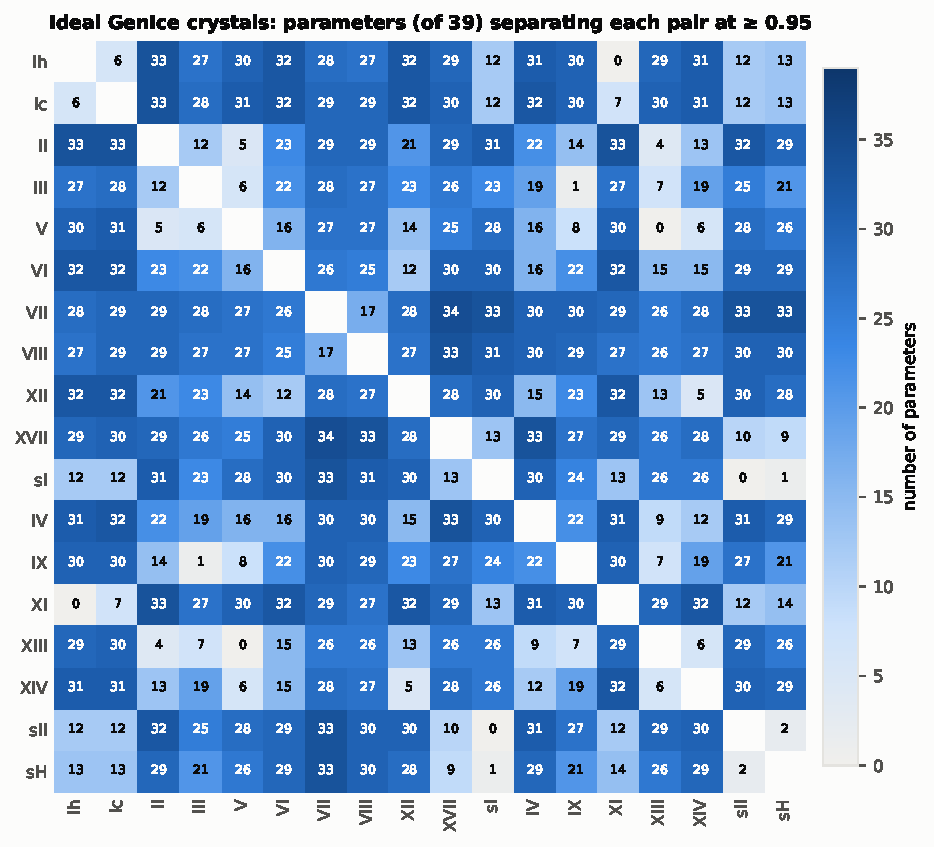
\includegraphics[width=.8\linewidth]{../benchmarks/results/figures/F1a_separability_ideal.pdf}
\caption{Number of parameters (of 39) that separate each pair of ideal
crystals with an oracle score of at least 0.95. The full parameter $\times$
pair matrix is in the Supplementary Information
(S1\_separability\_ideal\_all\_pairs).}
\label{fig:sep-ideal}
\end{figure}

\paragraph{Thermal and quenched structures.} At 220~K the picture changes
(Fig.~\ref{fig:sep-thermal}). For ice versus liquid, the best parameters are
locally averaged: $\bar s$ (1.00), $\bar q_6$ (0.99) and $\bar Q$ (0.98),
compared with 0.85, 0.78 and 0.84 for their unaveraged forms. The 6-ring
fraction (0.99) is the best unaveraged parameter. The cutoff coordination
number (0.62) and $N_\mathrm{HB}$ (0.53) are nearly useless. Energy
minimization restores most of the separation removed by thermal motion:
$d_5$, LSI and $\zeta$ rise from 0.83--0.84 to 1.00.

Ih and Ic are separated at 220~K only by $\bar q_3$ (1.00), $\bar q_4$
(1.00), $F_4$ (0.94), crystalline connections (0.93), $\bar q_6$ (0.78) and
CSP (0.72). Every other parameter is at 0.61 or below. Ring statistics cannot
distinguish them, since both contain only 6-rings. $\bar s$ separates Ih from
Ic perfectly in ideal crystals but only at 0.61 at 220~K.

\begin{figure}[H]
\centering
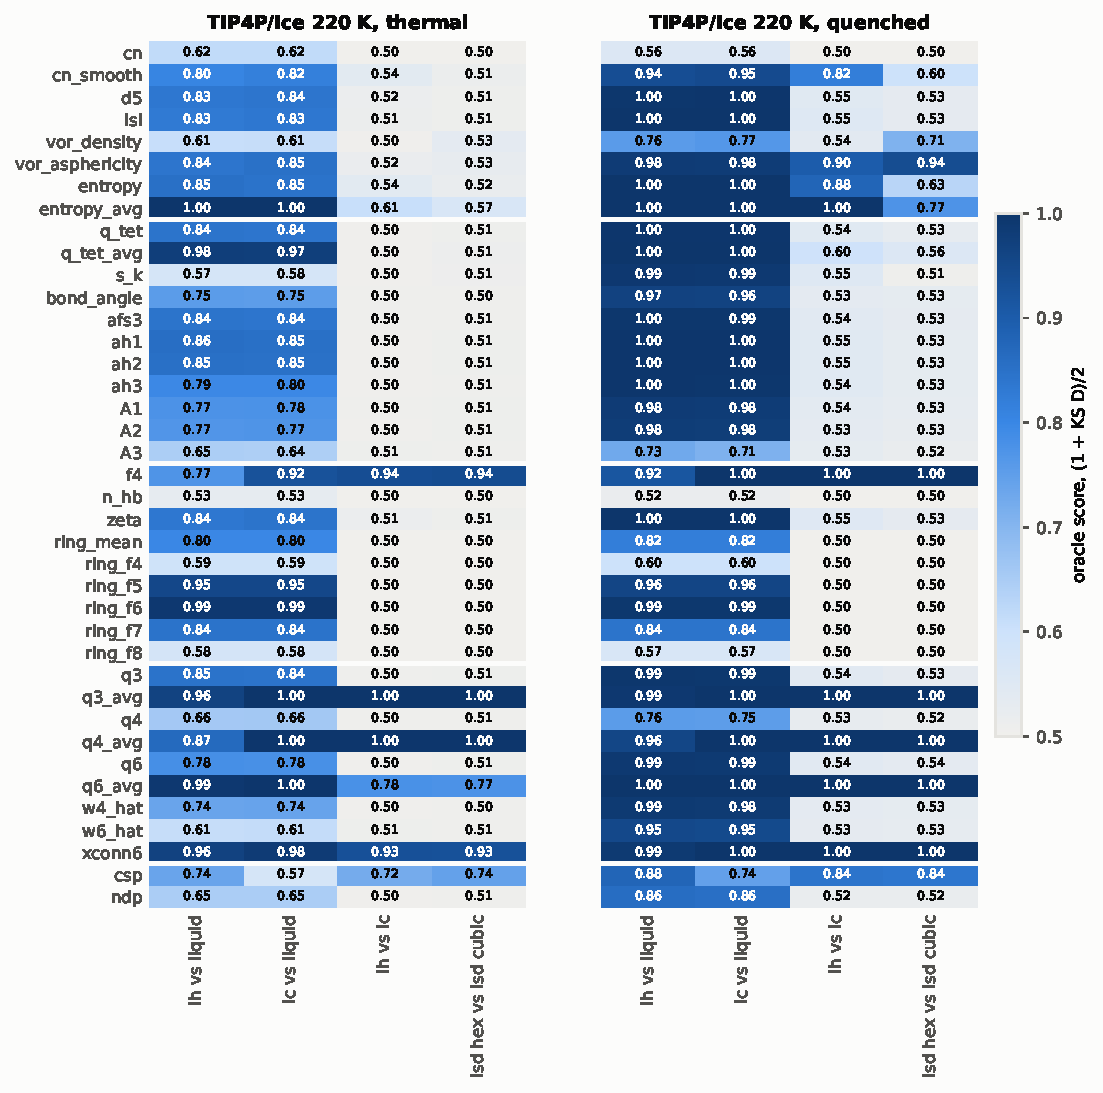
\includegraphics[width=.95\linewidth]{../benchmarks/results/figures/F1b_separability_thermal.pdf}
\caption{Oracle score $(1+D)/2$ for ice versus liquid, Ih
versus Ic, and hexagonal versus cubic layers in stacking-disordered ice,
TIP4P/Ice at 220~K. Left: thermal frames; right: the same frames after
energy minimization.}
\label{fig:sep-thermal}
\end{figure}

\paragraph{Held-out thresholds.}\label{sec:heldout} A threshold and its
direction fitted on run~A and applied to run~B lose at most 0.008 in balanced
accuracy relative to the oracle score on run~B, for every parameter and every
population pair, thermal or quenched (Fig.~\ref{fig:heldout}a). Fitting on
run~B and testing on run~A loses at most 0.011, and fitting on the first half
of run~B and testing on the second half at most 0.005. With $10^4$--$10^5$
molecules per population, a single fitted threshold barely overfits, and the
best parameter for each task is the same under both scores. Missing values
count as errors in the held-out scores; no parameter has any in these data.

What matters more is which populations are compared. Between runs, oracle
scores for Ih versus Ic agree within 0.013. With the bulk liquid of run~B
instead of the far liquid of run~A, 25 of 156 ice/liquid scores change by
more than 0.01, all of them distance- or density-based parameters (CN, smooth
CN, $d_5$, Voronoi, bond angle, $A_1$, $A_2$, CSP, neighbor distance), by up
to 0.05. At 250~K, Ih and Ic are still separated by $\bar q_3$ (1.00),
$\bar q_4$ (0.99), $F_4$ (0.91) and crystalline connections (0.88);
thresholds fitted at 220~K lose at most 0.03, for $\bar s$, which is weak
for this pair anyway (Fig.~\ref{fig:heldout}b).

Frame-to-frame correlation of per-frame means at 5~ps spacing is small in the
bulk crystals (median lag-1 autocorrelation $|r|<0.2$) but reaches 0.55 for
ring fractions in the liquid, so the intervals use blocks of five frames
(25~ps). Those intervals are narrow (median width 0.002) because they
describe one run. The between-run differences above are the better measure
of uncertainty.

\paragraph{Independent preparations.} Across the five preparations, oracle
scores vary little: the median standard deviation is 0.001, at most 0.008 for
thermal frames outside stacking-disordered ice and 0.016 within it
(Fig.~\ref{fig:grouped}). For every task whose mean oracle score is at least
0.8, leaving one preparation out costs at most 0.001, and thresholds fitted
on the seed test (run~A) cost at most 0.003 on any preparation. The best
parameters and their scores are unchanged: $\bar s$ 0.999 and $\bar q_6$
0.992 for Ih versus liquid; $\bar q_3$ 1.000, $\bar q_4$ 0.997, $F_4$ 0.938
and crystalline connections 0.924 for Ih versus Ic.

The exceptions are weak separations. Scores below 0.65 can fail to transfer:
in quenched stacking-disordered ice, smooth CN separates hexagonal from cubic
layers at 0.60 in one preparation but 0.51--0.52 in the other four, and a
threshold fitted on four preparations scores 0.45 on the fifth. The stacking
sequence, not the parameter, produced that separation. Hydrogen-aware
parameters score within 0.009 of each other in the polarized run~A crystals
and the unpolarized preparations, so the net dipole of the original crystals
does not affect them.

\paragraph{Second water model.}\label{sec:model} Thermal frames transfer
between models (Fig.~\ref{fig:model}). From TIP4P/Ice to TIP4P/2005, oracle
scores change by a median 0.004 (at most 0.025), at the same temperature or
the same undercooling, and wherever the oracle score is at least 0.8 a
threshold fitted on TIP4P/Ice loses at most 0.033 on the worst TIP4P/2005
preparation; only smooth CN loses more than 0.02. Changing the protocol from
the constructed constant-volume box to NPT costs at most 0.012. Quenched
frames are the exception. Their distributions are so narrow that the best
threshold sits at a model-specific value, and a small shift moves the whole
population across it: smooth CN and Voronoi density keep oracle scores of
0.97 and 0.82 for ice versus liquid in either model, but thresholds moved
from TIP4P/Ice score 0.47--0.65 on TIP4P/2005; MALIO $A_1$ and $A_2$ drop to
0.89--0.97. The same narrowness turns small density differences into
spurious structure: under NPT, Ic is 0.35\% denser than Ih, and that alone
gives Voronoi density and neighbor-distance ($D$) oracle scores of 0.74--0.90 for quenched Ih
versus Ic, compared with 0.52--0.55 in the fixed run~C box. Rankings and the
best parameters ($\bar s$, $\bar q_6$, $\bar q_3$, $F_4$) do not change.

The oxygen-only mW model is a harder test (Fig.~\ref{fig:model}d). The
leading parameters still transfer within 0.01: for ice versus liquid,
$\bar s$ (1.000), $\bar q_6$ (0.998), $\bar Q$ (0.991) and $\bar q_3$ (0.987);
for Ih versus Ic, $\bar q_3$ and $\bar q_4$ ($\ge 0.998$). But here
first-shell distance parameters fail to transfer even in thermal frames,
because the mW liquid packs more neighbors into the first shell (median
smooth CN 4.76 against 4.39 for TIP4P/Ice). Smooth CN separates ice from mW
liquid with an oracle score of 0.90 but scores 0.67 with the TIP4P/Ice
threshold; $A_1$ drops from 0.80 to 0.72, $d_5$ and LSI lose about 0.04, and
$\bar q_6$ for Ih versus Ic drops from 0.87 to 0.81. Several distance-based
parameters separate ice from liquid better in mW (CN 0.63 to 0.79, $D$ 0.59
to 0.80, $d_5$ 0.87 to 0.92), and Voronoi density worse (0.68 to 0.58). In
quenched frames, smooth CN, Voronoi density and asphericity, entropy and $D$
separate mW Ih from Ic almost perfectly ($\ge 0.998$, against 0.57--0.95 for
TIP4P/Ice). Without proton disorder the quenched crystals are nearly perfect
lattices, and the 0.4\% density difference between Ih and Ic in NPT is
enough to separate them; that is not a stacking signal.

\paragraph{High-pressure phases.}\label{sec:pressure} Every pair of the eight
crystals is still separated by some single parameter at 220~K
(Fig.~\ref{fig:pressure}a): the best held-out score, taking the worse of the
two preparations, is at least 0.98 for every pair except VII/VIII, where
$\bar q_6$ reaches 0.92 (1.00 for quenched frames, through the angle
histogram). Individual parameters suffer much more than this best case
(Fig.~\ref{fig:pressure}b). Of the 684 crystal pair and parameter
combinations with an ideal oracle score of at least 0.95, 31\% fall below
0.95 and 10\% below 0.8 in thermal frames; quenching restores all but 3.5\%.
Losses are largest for $\hat w_4$ and $\hat w_6$ (median 0.23--0.26), neighbor distance $D$
(0.14), and unaveraged $q_6$, $F_4$ and entropy (0.06--0.08), and near zero
for the averaged and network parameters. Averaged entropy separates
crystal pairs best on average (mean held-out 0.96), followed by smooth CN,
Voronoi asphericity and $\bar Q$ (0.94).

The hard tasks are high-pressure ice against compressed liquid. Ice~V
against liquid at 0.3~GPa reaches only 0.85 with the best parameter
(Voronoi asphericity), III against ambient liquid 0.94, II against liquid at
0.3~GPa 0.97, and liquids at different pressures 0.85--0.99. No parameter
separates every high-pressure ice from every liquid: the best worst case is
$\bar Q$ at 0.65. Ice-versus-liquid recommendations from ambient pressure do
not carry over. Thresholds also become fragile in quenched frames here: 62
quenched pair and parameter scores at or above 0.8 lose more than 0.02
between the two preparations (one in thermal frames), mostly for ices II and
VIII with $d_5$, $\bar s$, smooth CN, $\zeta$ and Voronoi density. Quenched
ordered crystals have nearly delta-shaped distributions ($d_5$ standard
deviation 0.0002--0.003~\AA), and the two preparations differ by their final
box (0.4\% in density for ice II), which moves the peaks by more than their
width.

\begin{figure}[H]
\centering
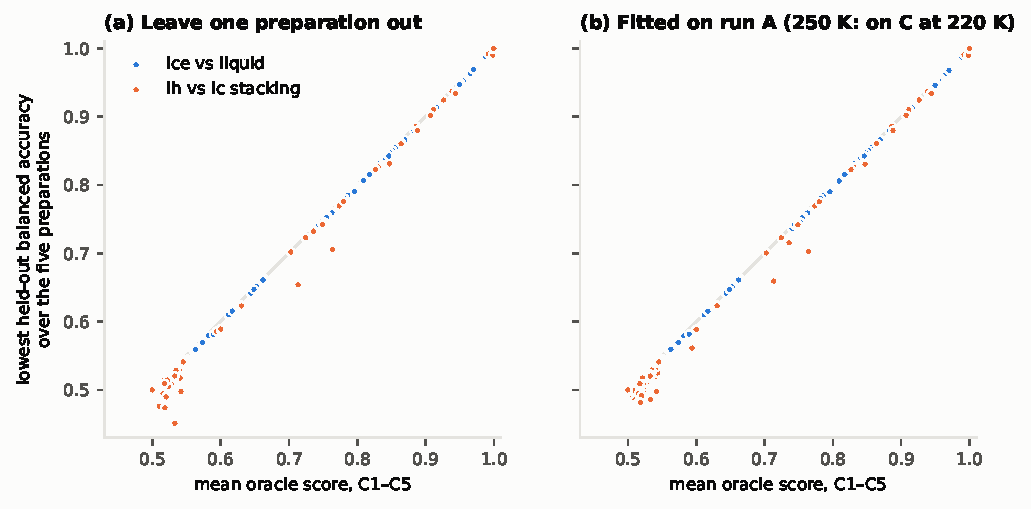
\includegraphics[width=.95\linewidth]{../benchmarks/results/figures/S3_grouped.pdf}
\caption{Five independent preparations (C1--C5). Each point is one parameter
and population pair, thermal and quenched; vertical axis: lowest held-out
balanced accuracy over the five preparations. (a) Threshold fitted on the
other four preparations. (b) Threshold fitted on the seed test (run~A); for
Ih versus Ic at 250~K, on the 220~K preparations.}
\label{fig:grouped}
\end{figure}

\begin{figure}[H]
\centering
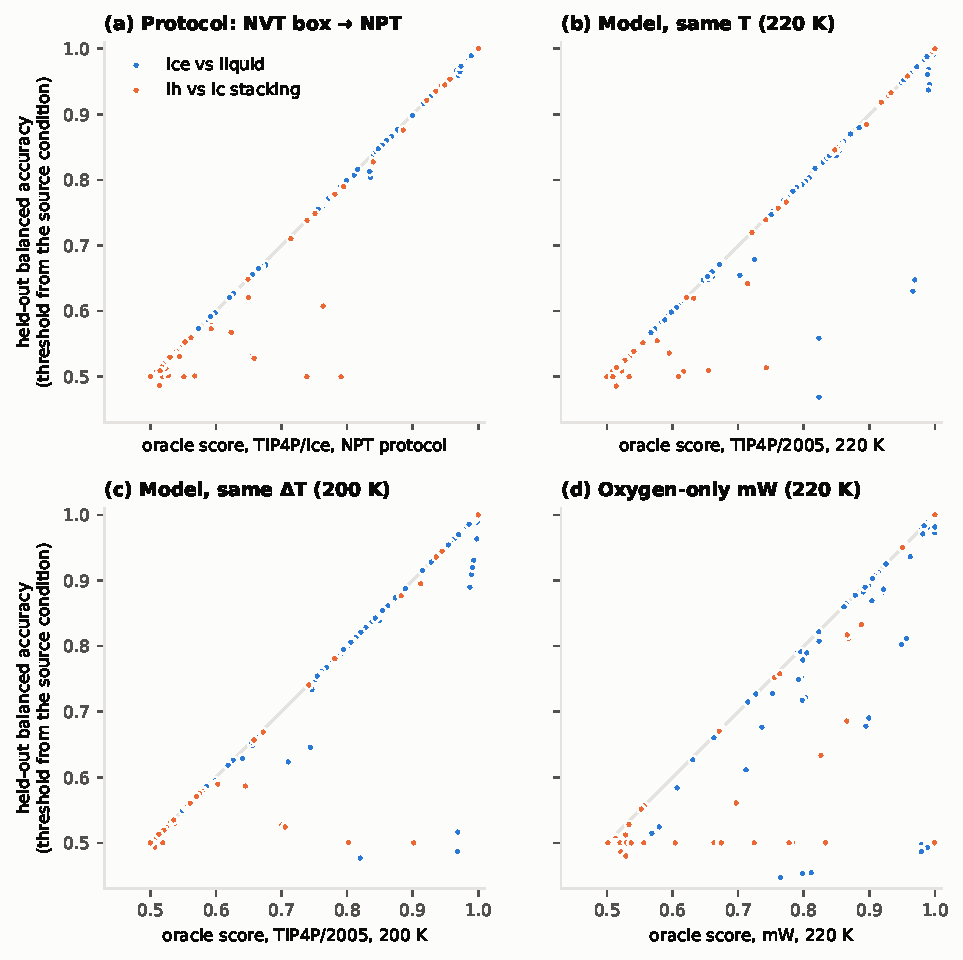
\includegraphics[width=\linewidth]{../benchmarks/results/figures/S4_model.pdf}
\caption{Moving thresholds between protocols and water models (run~D). Each
point is one parameter and population pair, thermal and quenched; horizontal
axis: oracle score on the target condition; vertical axis: held-out score of
the threshold fitted on the source condition, preparations pooled. (a)
TIP4P/Ice, constructed constant-volume box (run~C) to the NPT protocol. (b,c)
TIP4P/Ice to TIP4P/2005 at 220~K and at 200~K. (d) TIP4P/Ice to mW at
220~K; hydrogen-dependent parameters are absent. The outliers far below the
diagonal are distance- and density-based parameters, in quenched frames for
TIP4P/2005 and also in thermal frames for mW.}
\label{fig:model}
\end{figure}

\begin{figure}[H]
\centering
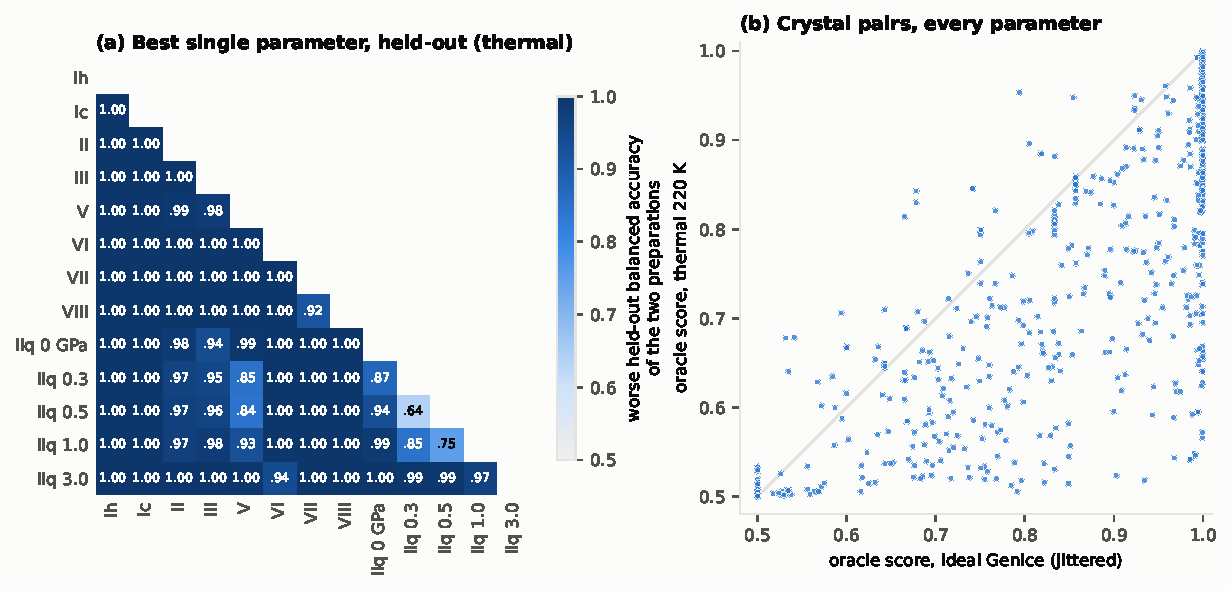
\includegraphics[width=\linewidth]{../benchmarks/results/figures/F8_pressure.pdf}
\caption{Thermal high-pressure phases, TIP4P/Ice at 220~K (run~E). (a) Best
single parameter per pair, scored by the worse of the two held-out
directions between preparations; liquids at 0, 0.3 and 1.0~GPa. (b) Every
parameter and crystal pair: oracle score of the ideal, jittered GenIce
structures against the thermal oracle score.}
\label{fig:pressure}
\end{figure}

\begin{figure}[H]
\centering
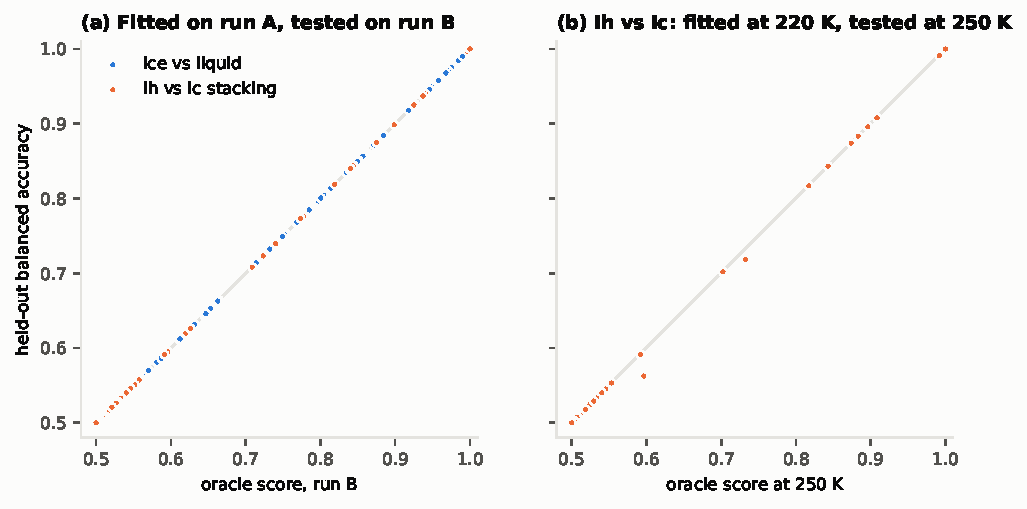
\includegraphics[width=.95\linewidth]{../benchmarks/results/figures/S2_heldout.pdf}
\caption{Held-out against oracle scores, one point per parameter and
population pair (thermal and quenched). (a) Threshold fitted on run~A,
balanced accuracy on run~B, at 220~K. (b) Ih versus Ic in run~B: threshold
fitted at 220~K, balanced accuracy at 250~K. Points on the diagonal lose
nothing.}
\label{fig:heldout}
\end{figure}

\paragraph{Redundancy.} Many parameters carry nearly the same information.
Grouping parameters whose Spearman rank correlation exceeds 0.8 in absolute
value reduces the 39 columns to 22 groups (Fig.~\ref{fig:redundancy}). The
largest group joins $Q$, the bond angle, the angular Fourier term, the
three angle-histogram amplitudes, $q_3$, $q_6$ and $\hat w_4$. Other groups
join $\bar q_3$, $\bar q_4$, $\bar q_6$ and crystalline connections; $d_5$,
LSI, $s$ and $\zeta$; $\bar Q$ and $\bar s$; and the 5- and 6-ring
fractions.

\begin{figure}[H]
\centering
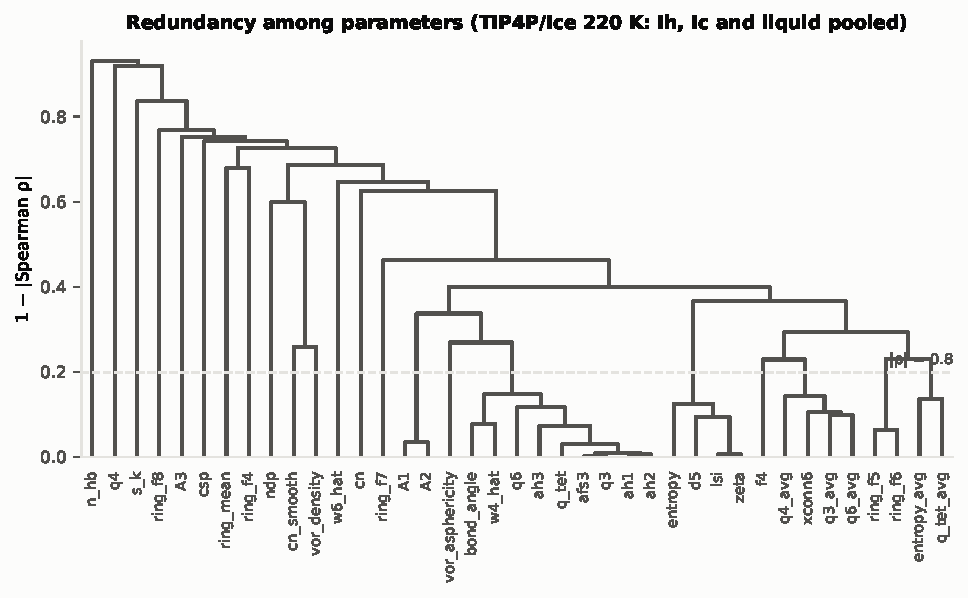
\includegraphics[width=.95\linewidth]{../benchmarks/results/figures/F2_redundancy.pdf}
\caption{Hierarchical clustering of parameters by $1-|\rho|$, with $\rho$ the
Spearman correlation over thermal Ih, Ic and liquid molecules at 220~K. The
dashed line marks $|\rho| = 0.8$.}
\label{fig:redundancy}
\end{figure}

\section{Ice labelers against ground truth}
CHILL+ labels 99.7\% of thermal bulk Ih correctly, while the original CHILL
labels only 70.7\%. The eclipsed-bond window is the reason. In thermal bulk
Ih, every four-coordinated molecule keeps its three staggered bonds, but the
correlation of its eclipsed bond falls inside CHILL's window $(-0.2,-0.05)$
for only 70.8\% of molecules (5th--95th percentile $-0.23$ to $0.01$),
against 100\% for CHILL+'s $(-0.35, 0.25)$~\cite{Nguyen2014}. After energy
minimization both windows contain every eclipsed bond. PTM with the default
RMSD cutoff labels 97\% of bulk ice correctly and never labels liquid as ice.
False-positive rates in the far liquid are at most 1\% for all three
labelers.

In the seeds, all three recover only part of the constructed crystal
(Fig.~\ref{fig:labels}): CHILL+ finds 11\% of interior molecules of a
50-molecule Ih seed with the correct polytype, and 58\% for a 200-molecule
seed. Construction labels describe the starting structure, so we audited each
frame before reading these numbers as errors. A seed molecule counts as
intact when it lies within 1~\AA{} of its constructed site (after removing
the seed's drift) and keeps all its constructed bonds shorter than
3.5~\AA. In the 100- and 200-molecule seeds 81--90\% of seed molecules are
intact (94--99\% of interior ones). The 50-molecule Ih seed is the most
deformed: 57\% intact, 75\% of its interior.

Recall depends on depth below the constructed seed surface, and hardly on
seed size or polytype (Fig.~\ref{fig:depth}). CHILL+ finds the correct
polytype for at most 15\% of molecules within 3~\AA{} of the surface, about
70\% at 4--5~\AA{} and over 90\% beyond 6~\AA, although about 90\% of
molecules are intact already at 2--4~\AA{} depth. Between 1 and 4~\AA{} it
puts 17--58\% of molecules in its separate interfacial-ice class instead. A
50-molecule seed ($R \approx 7.3$~\AA) has only 3--4\% of its molecules deeper
than 5~\AA, which explains most of its low score; for the Ih seed, real
deformation adds to it. PTM needs about 2~\AA{} more depth. Its best
diamond-template RMSD falls below the default cutoff of 0.1 for half of the
molecules only at 6--7~\AA{} depth (median 0.07--0.09 deep inside a seed,
0.12--0.14 at 4--5~\AA). CHILL is below CHILL+ for Ih and stacking-disordered
seeds at most depths, as in bulk Ih; for Ic seeds it is level or slightly
ahead. Small-seed recall therefore measures how much crystalline support
each labeler needs around a molecule, not only whether it recognizes ice.

\begin{figure}[H]
\centering
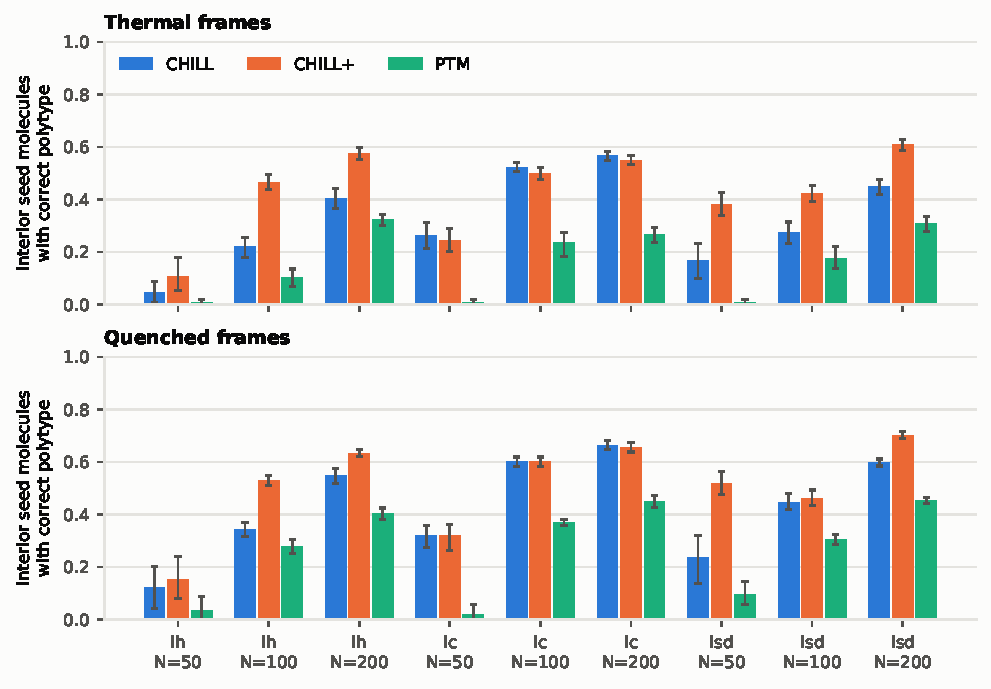
\includegraphics[width=.95\linewidth]{../benchmarks/results/figures/F7_seed_labels.pdf}
\caption{Fraction of interior seed molecules labeled with the correct
polytype by CHILL, CHILL+ and PTM, for Ih, Ic and stacking-disordered (Isd)
seeds of $N$ molecules in TIP4P/Ice liquid at 220~K. Error bars: 95\%
bootstrap intervals over frames.}
\label{fig:labels}
\end{figure}

\begin{figure}[H]
\centering
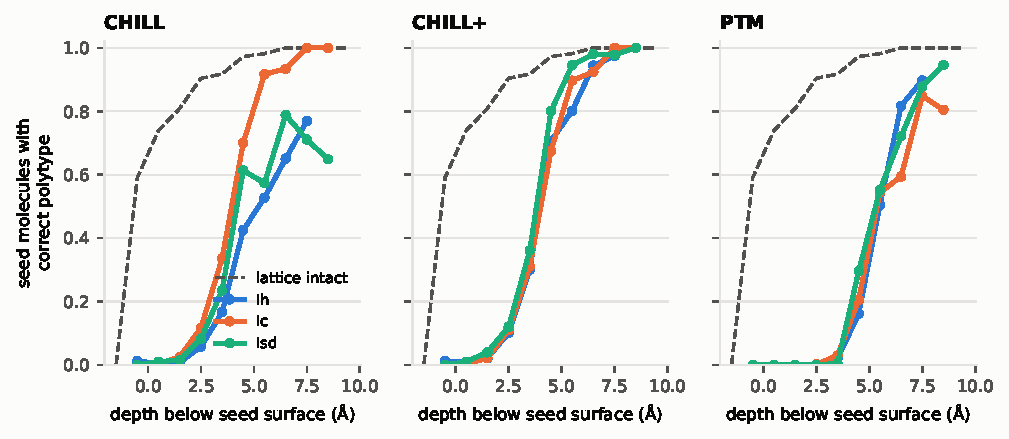
\includegraphics[width=.95\linewidth]{../benchmarks/results/figures/F7b_seed_depth.pdf}
\caption{Fraction of seed molecules labeled with the correct polytype against
depth below the constructed seed surface, $R - r$, pooled over seed sizes,
thermal frames at 220~K. Dashed: fraction of molecules whose constructed
lattice is intact (within 1~\AA{} of the constructed site, all constructed
bonds kept). Bins with fewer than 30 molecules are omitted.}
\label{fig:depth}
\end{figure}

\todo{Caveats to state: run~A frames are 1~ps apart, so its bootstrap
intervals are too narrow; both liquid references are supercooled;
ideal-crystal results depend on GenIce cell geometries.}

\section{Sensitivity to neighbor definition and water model}
TIP4P/Ice versus TIP4P/2005 and mW is in Sec.~\ref{sec:model}: averaged
and angular parameters transfer; first-shell distance and density parameters
do not, in quenched frames between the TIP4P models and also in thermal
frames for mW.
\plan{Cutoff scans; $N$-nearest vs.\ cutoff.}

\section{Computational cost}
\plan{Time per molecule vs.\ system size, serial and parallel.}
\code{n\_jobs and backend options (parallel.py).}

\section{Application: following an interface or nucleation event}
\plan{Per-molecule labels along one trajectory from CHILL+, $q_6$-based,
PTM and a descriptor-based method; agreement and disagreement.}

%=====================================================================
\chapter{Practical guide}\label{ch:guide}
%=====================================================================
\plan{Decision table: question (ice vs.\ liquid, Ih vs.\ Ic, hydrate vs.\ ice,
high-pressure polymorphs, collective variable for sampling) $\rightarrow$
recommended parameter(s), settings and caveats.}

\begin{table}[H]
\centering
\small
\caption{Provisional recommendations from the benchmark so far (ideal
crystals; TIP4P/Ice at 220~K, Ih/Ic also at 250~K, up to seven runs, five of them
independent preparations; TIP4P/2005 at 220 and 200~K; mW at 220~K; six
high-pressure ices and compressed liquid at 220~K). Rankings are the same for
oracle and held-out scores; treat any separation below ${\sim}0.65$ as
preparation-specific, and do not move thresholds of distance- or
density-based parameters between models or boxes.}
\label{tab:guide}
\begin{tabular}{p{.27\linewidth}p{.33\linewidth}p{.3\linewidth}}
\toprule
Question & Best so far & Avoid \\
\midrule
Ice vs.\ liquid, ambient & $\bar s$, $\bar q_6$, $\bar Q$; 6-ring fraction if no
averaging is wanted & CN, $N_\mathrm{HB}$ \\
Ih vs.\ Ic & $\bar q_3$, $\bar q_4$; $F_4$ if hydrogens are available & ring
statistics, unaveraged parameters \\
Per-molecule labels in seeds & CHILL+ (Ih, stacking-disordered), CHILL or
CHILL+ (Ic); expect reliable labels only ${\gtrsim}6$~\AA{} inside a
crystal & CHILL for Ih; PTM within ${\sim}7$~\AA{} of an interface \\
Distinguishing crystal phases & $\bar s$, smooth CN, Voronoi asphericity,
$\bar Q$; $\bar q_6$ or $\bar q_4$ for VII/VIII & $\hat w_4$, $\hat w_6$,
$D$, $N_\mathrm{HB}$, $A_3$ \\
High-pressure ice vs.\ compressed liquid & per pair (Fig.~\ref{fig:pressure});
no single parameter above 0.65 for all & ambient-pressure choices without
checking \\
Proton-ordered vs.\ disordered & no local parameter tested is reliable
(VII/VIII separate through their oxygen lattices) &
-- \\
\bottomrule
\end{tabular}
\end{table}

\section{Software}
\plan{SolOrder alongside freud, OVITO, PLUMED, pyscal and MDAnalysis:
coverage, parallelism, differentiability, licensing.}

\section{Reproducibility checklist}
\plan{What to report when using an LOP: neighbor rule, cutoff, averaging,
water model, thresholds and their calibration.}

%=====================================================================
\chapter{Outlook}\label{ch:outlook}
%=====================================================================
\plan{Open problems: proton-ordered partners, amorphous ices, interfaces and
confinement, transferability of learned models across water models, LOPs as
differentiable CVs.}

\section*{Data and code availability}
\plan{SolOrder version, benchmark scripts and datasets (DOI).}

\section*{Acknowledgments}
\plan{Funding, computing resources.}
% basic/ack.tex is a thesis declaration and is not used in the review.

% Previous chapter files, kept for reference while rewriting:
% \chapter{Introduction}
\pagenumbering{arabic} \setcounter{page}{1}

Ice, which is formed from the freezing of water, is one of the most ubiquitous substances on Earth, and yet it exhibits a remarkable diversity of molecular geometries depending on temperature and pressure\cite{Zheligovskaya2006}. In fact, scientists have identified at least 20 crystaline phases of ice, each with its own unique crystal structure and properties\cite{BartelsRausch2012}\cite{Fuentes-Landete}. There exists three amorphous phases of ice on top of the crystal ones\cite{Fuentes-Landete}. Understanding the characteristics of these different forms of ice is crucial for multiple scientific fields, including climate science and materials science, as it provides valuable insights into their behavior and properties.\\
The most familiar form of ice is Ice-Ih, which has a hexagonal crystal structure and interlocking hydrogen bonds between water molecules. This form of ice is what we typically encounter in our daily lives, such as in snowflakes and ice cubes\cite{Baker2019}. Conversely, Ice-II has a rhombohedral crystal structure and higher density than Ice-Ih and forms under high pressures and low temperatures\cite{Kamb1964}. Ice-III can exist at temperatures as low as $-100 \degree C$ and under greater pressures than Ice-II, making it useful in high-pressure experiments\cite{Bauer_2008}. Ice-V is one of the densest form of ice, characterized by its monoclinic crystal structure, forms at 253K temperature and 500MPa\cite{Hasted_1969}. Similarly, Ice-VI is denser than Ice-III and forms under high pressures and low temperatures, providing insights into planetary science\cite{Kuhs_1984}. Ice-VII is a cubic crystal form of ice with a unique crystal structure and properties that are still being studied\cite{Kuhs_1984}.\\
Cubic ice, or Ice Ic, assumes a cubic shape and has different hydrogen bonding than other forms of ice\cite{Murray_2006}. Clathrate structures, which form when gas molecules are trapped within the ice lattice, are crucial in the study of gas hydrates, the storage and release of methane from the ocean floor, and the Earth's climate\cite{Buffett2004}\cite{Buchanan2005}. The classification of these packing geometries has been achieved through considerable effort in molecular structure analysis. While conventional crystallographic analysis has been used, current molecular simulation shows promise in providing precise real-space geometrical information for many molecular systems. However, molecular geometry classification remains a challenging task. To efficiently distinguish between different structures, order parameters are often utilized\cite{CHAU_1998}\cite{Giovambattista_2005}\cite{Yan_2007}\cite{Zimmermann2017}\cite{Yan2007}\cite{Errington2001}\cite{Piaggi2017}\cite{Lechner2008}\cite{Reinhardt2012}\cite{Mickel2013}. Moreover, order parameters can be defined for local structures to describe transient structures during phase transitions.\\
The structure of ice is of great interest as it exhibits a wide range of fascinating properties, such as high thermal stability, unique optical and electronic properties, and important implications in climate science. The regular lattice of water molecules forming a tetrahedral arrangement through hydrogen-bond interactions characterizes the structure of ice, while the local structure of liquid water lacks long-range order, and only a partial short-range order remains, influenced by various factors such as pressure, temperature, solutes, and hydrophobic groups\cite{Galamba_2013}. By gaining a deeper understanding of the molecular geometries of ice, scientists can better understand the behavior and properties of this vital substance, with potential applications in fields such as materials science, energy storage, and climate modeling.\\
The intricate phase space of ice and water gives rise to a multitude of transitions across various phases\cite{Hansen2021}\cite{Chaplin2019}\cite{Bore2022}\cite{Hirata2017}. These transitions encompass a wide spectrum of direct-indirect and ordered-disordered phenomena, which poses a considerable challenge in molecular simulation due to the vastness of the configuration space. The need for a mathematical functional, specifically an order parameter, becomes imperative to effectively describe these phenomena and capture the nuanced microscopic events occurring.\\
However, this task becomes considerably complex owing to the subtle differentiations existing across different phases. Sometimes, the similarities are so intricate that they cannot be discerned using simple geometric functions\cite{Moore2011}. While researchers have leveraged their domain knowledge to devise such order parameters, they tend to be highly specific to individual cases and often require computationally intensive calculations.

\begin{figure}[H]
\centering
\includegraphics*[width=.85\linewidth]{intro/phase.png}
  \caption{Phases labeled with black Roman numerals are hydrogen-disordered phases; those labeled with red numerals are hydrogen-ordered phases; those labeled with blue numerals are metastable phases. The red solid arrows represent direct disorder-order transitions. The red dotted arrows represent disorder-order transitions that cross the stability range of another phase\cite{Hansen2021}.}
\label{fig:Phase diagram}
\end{figure}
Among the widely utilized order parameters is the tetrahedral order parameter, extensively employed to probe local structures around water molecules and their hydrogen bonding networks. Ranging from 1 for a pure tetrahedral network to approaching 0 for random configurations, this parameter offers insight into the local environment\cite{CHAU_1998}\cite{Galamba_2013}\cite{Giovambattista_2005}\cite{Yan2007}.
In distinguishing between clathrates and bulk water, the four-body structural order parameters ($F_4$) have gained popularity. By considering the dihedral formed by two neighboring oxygen atoms (within a defined cutoff) and two outward hydrogen atoms attached to the oxygen molecules,the $F_4$ parameters provide valuable discrimination\cite{Rodger1996}.
Recent trends highlight the utility of entropy fingerprints and their localized counterpart, the local entropy\cite{Piaggi2017} . By employing the radial distribution function, these methods capture the fluctuation of conformations with significant success.
An intuitive approach to address this challenge traditionally revolves around the introduction of bond orientational order parameters. These parameters, based on rotationally invariant spherical harmonics, have found success in describing crystallization events. Steinhardt's order parameters, in particular, have been instrumental in distinguishing various ice phases based on their characteristic order parameter distributions\cite{Plimpton1995}.
A more intricate approach involves the utilization of atom-centered symmetry functions\cite{Behler2011}. With a unique atomic descriptor generated for the distribution of particles in 3D, the Smooth Overlap of Atomic Positions (SOAP) technique stands out\cite{De2016}\cite{Maksimov2020}. SOAP offers a local descriptor that meticulously encapsulates the subtle details of the immediate spatial environment surrounding a specific point. Through Gaussian smearing and transformation into coefficients using an orthonormal basis function system, SOAP effectively mitigates redundancies associated with rotation, translational, and permutation\cite{Himanen2020}.\\
However, despite these efforts, the design of physical intuition-based order parameters remains challenging. They tend to be specific to particular systems, computationally demanding, and may sometimes overlook valuable concealed information\cite{Donkor2023}\cite{Fulford2019}\cite{Doi2021}. In response to these challenges, the last decade has witnessed a surge in the utilization of Machine Learning (ML) methods. Data-driven models are now being employed to identify various local patterns present in simulation snapshots. Leveraging the capacity of deep neural networks to uncover hidden patterns within seemingly random distributions has paved the way for a new era in order parameter exploration..   
In recent years, the landscape of order parameter exploration has been dramatically expanded by the advent of various Machine Learning (ML) approaches\cite{ML_Method1}\cite{Cheng2019}. Convolutional Neural Networks (CNNs) have demonstrated remarkable proficiency in capturing spatial patterns within simulation snapshots\cite{Li2022}. These networks, often utilized in image recognition tasks, have been adapted to analyze the structural arrangements of molecules.
Graph Neural Networks (GNNs) provide an ideal framework for dealing with molecular systems, where atoms and their interactions can be represented as nodes and edges within a graph. GNNs excel at capturing complex dependencies and interactions, making them particularly suited for identifying structural motifs within simulations\cite{Hofstetter2022}\cite{Kim2020}.
Autoencoders, a type of neural network architecture, facilitate the extraction of lower-dimensional representations from high-dimensional data. They are adept at discerning latent features and structural characteristics that may not be immediately apparent in the original data. By training on simulation snapshots, autoencoders can uncover hidden relationships and patterns within the molecular configurations\cite{Kim2020}.
Incorporating these ML methods has revolutionized the study of order parameters, enabling the discovery of intricate correlations and complex structural changes that were previously elusive. As our understanding of ML techniques deepens, they promise to further enrich our insights into the phase transitions and behaviors of ice and water, unveiling hidden intricacies that were once beyond our grasp.\\
In this study, the local structure of various ice phases is investigated, and several order parameters are calculated to characterize them. A range of geometric order parameters, including orientational and translational tetrahedral order parameters, local structure index, local density based on Voronoi polyhedra, asphericity of the Voronoi cell, water-water angular distribution function, and Steinhardt’s bond orientational order parameter etc. have been proposed to quantify the local structure of ice phases. Our aim is to provide a comprehensive understanding of the local structure of different ice phases and the performance of various order parameters in characterizing them.



% \chapter{Various Ice Phases}\label{ch:icephases}
Approximately twenty distinct three-dimensional crystalline phases exist, each characterized by specific arrangements of oxygen atoms in fixed positional relationships\cite{BartelsRausch2012}\cite{Fuentes-Landete}. The disposition of hydrogen atoms within these phases can vary, introducing the possibility of disorder. Concurrently, there are three amorphous (non-crystalline) phases, along with a multitude of computer-simulated ices that have been postulated theoretically. This profusion of ice phases can be attributed to the inherent tetrahedral configuration of water molecules within hexagonal ice, a configuration that serves as the foundation for the diverse crystal structures which emerge as this ice is subjected to increasing pressure, ultimately leading to its compression.\\
\begin{figure}[H]
\centering
\includegraphics*[width=.8\linewidth]{background/unitcell.png}
  \caption{Representative ice unit cells(generated using GenIce software)}
\label{fig:Ice unit cells}
\end{figure}
In the realm of crystalline ice phases, a consistent feature involves the intricate interplay of hydrogen bonding between water molecules, with each water molecule engaging with four neighboring counterparts. Generally, the two hydrogen atoms within each molecule exhibit a degree of equivalence, resulting in hydrogen bonds of comparable strength. This symmetrical arrangement of water molecules adheres to the principles known as the 'ice rules'\cite{OrtizAmbriz2019}. Evidently, the propensity for proton ordering—fixed positions with a consequent reduction in entropy—occurs more prominently at lower temperatures. Contrasting this, elevated pressures serve to diminish the distances separating second shell neighbors, yielding a reduced volume accompanied by heightened van der Waals effects.\\
The structural characteristics of ice phases entail an anticipated H-O-H bond angle that slightly deviates from the perfect tetrahedral angle ($109.47 \degree$), hovering around $107\degree$. Importantly, the complexities of phase transitions in multiple ice forms demand a tailored adaptation of the Clausius-Clapeyron equation, prompted by water's idiosyncratic negative expansion coefficient and its anomalous alterations in entropy with varying volume\cite{Stepanov_2007}. This equation, an essential cornerstone of thermodynamics, must be recalibrated to effectively capture the nuanced behavior exhibited by water during these intricate phase change\\
\section{IceIh}
Hexagonal ice, denoted as Ice-Ih, is a fundamental crystalline phase of ice and is considered the most common naturally occurring form of ice\cite{Baker2019}. Its name originates from the hexagonal lattice arrangement that its water molecules adopt. The structure of hexagonal ice is defined by the intricate interplay of hydrogen bonds and the unique geometry of water molecules. In hexagonal ice, each water molecule is surrounded by four neighboring water molecules, forming a tetrahedral arrangement. The oxygen atoms of water molecules form the vertices of a hexagonal lattice, while the hydrogen atoms extend outwards from the oxygen atoms. These hydrogen atoms are engaged in hydrogen bonds with oxygen atoms of adjacent molecules, resulting in a highly stable and organized structure.
The angles between the hydrogen bonds in hexagonal ice are close to the ideal tetrahedral angle of $109.47\degree$, although they are slightly compressed to about $107\degree$ due to the constraints of the hexagonal lattice. This angle compression contributes to the characteristic hexagonal symmetry of the ice\cite{Pamuk2018}.\\

\begin{figure}[H]
\centering
\includegraphics*[width=.8\linewidth]{icephases/images/iceIh.png}
\caption{Representative snapshots of IceIh}
\label{fig:IceIh}
\end{figure}


Hexagonal ice exhibits distinct layers within its structure, with water molecules forming planar layers that stack on top of each other. The arrangement of these layers is such that each layer is shifted slightly relative to the layer below, leading to an "ABABAB" stacking pattern. This stacking pattern is another hallmark of hexagonal ice's structural arrangement.
While hexagonal ice is one of the most well-studied forms of ice, it serves as a cornerstone for understanding the complexities of water's behavior in various environments. The understanding of its structural details provides insights into the broader landscape of ice phases and their role in phenomena like glacial formation, climate dynamics, and the behavior of water on other planets.

\section{IceIc}
Cubic ice, or Ice-Ic, is a metastable ice crystal formed through condensation of water vapor under specific conditions: below $-80\degree C$ at ambient pressure, in small droplets below $-38\degree C$ \cite{Murray_2006}, or through pressure reduction on high-pressure ices at 77K \cite{Ji_2011}. It often acts as a transition state between hexagonal and cubic ice due to its structural variability. The initial ice from supercooled water is stacking-disordered, making its composition complex.\\
Cubic ice's unique characteristics include slightly lower melting points and slightly higher vapor pressures compared to ice Ih. It can form rare halos around the Sun in the upper atmosphere. It's prevalent in freezing confined aqueous systems. It's preferred for small water droplets ($<15 nm$ radius) due to lower interfacial free energy. Larger cubic ice crystals slowly and irreversibly convert to hexagonal ice with heat evolution.\\
\begin{figure}[H]
\centering
\includegraphics*[width=.8\linewidth]{icephases/images/iceIc.png}
\caption{Representative snapshots of IceIc}
\label{fig:IceIc}
\end{figure}
Structurally, cubic ice has a face-centered cubic lattice with half-filled tetrahedral holes. Pure cubic ice was discovered in 2020. Like Ice-Ih, it has a moderately open low-density structure with a packing efficiency of about 1/3. Unlike Ice-Ih, its hydrogen-bonding arrangement is staggered to all neighbors. Cubic ice's layers are identical and slightly displaced, maintaining similar density to Ice-Ih.
\section{IceII}
 Ice-II emerges through the synthesis of hexagonal ice at a temperature of 198 K and a pressure of 300 MPa. Another avenue for its creation involves decompressing Ice-V at 238 K, yet it doesn't readily form through the cooling of Ice-III. This distinctive phase is known to constitute a significant proportion of icy moons like Jupiter's Ganymede \cite{Fortes_2005}.\\
The defining characteristic of Ice-II lies in its systematically ordered arrangement of hydrogen bonds. Unlike other ordered ices, Ice-II lacks a disordered counterpart. Interestingly,when heated towards its melting point, it transitions into Ice-Ih, Ice-III, Ice-V, or Ice-VI. An intriguing aspect is that the presence of minute quantities of ammonium fluoride (e.g., 0.5 mol\% $NH_4^+ F^-$) disrupts the existence of Ice-II from water's phase diagram, acting as a hydrogen-disordering agent\cite{Shephard_2018}.\\
The unit cell of Ice-II forms rhombohedral crystals, falling under the space group $R\bar{3}$. Within the crystal lattice, each water molecule establishes hydrogen bonds with four others - two as donors and two as acceptors. Ice-II can exist in a metastable state at temperatures below $\equiv$ 100 K between ambient pressure and $\equiv$ 5 GPa. However, at ambient pressure, a transformation into Ice-Ic takes place irreversibly above 160 K.
\begin{figure}[H]
\centering
\includegraphics*[width=.8\linewidth]{icephases/images/ice2_3.png}
\caption{Representative snapshots of IceII}
\label{fig:IceII}
\end{figure}

Ice-II is characterized by collapsed open hexagonal channels, a departure from Ice Ih. Its structural relationship to ice Ih can be conceptualized by detaching the columns of hexameric ice Ih rings, vertically displacing them while maintaining a right angle to their plane, rotating them around a $30 \degree$ axis, and then reconfiguring the hydrogen bonds in a more compact manner. This intricate process yields a density of $1.16 g.cm^-3$ \cite{Nakamura2015}. The hydrogen bonding within Ice-II is impeccably ordered and fixed, a feature evident in the connections surrounding the hexamers. Unlike other ordered ices like Ice-VIII, Ice-IX, Ice-XI, and Ice-XV, there is no corresponding disordered phase in Ice-II. While speculative disordered forms of Ice-II have been explored, they exhibit reduced stability due to higher Gibbs free energy and zero-point energy. Nonetheless, the possibility of partial hydrogen-bond disorder within actual Ice-II remains. This unique absence of a disordered phase can be attributed to the notable energy gap between the most and second most stable ice configurations \cite{Fan_2010}. Some hydrogen bonds within Ice-II appear bent, resulting in a weakened strength in comparison to the hydrogen bonds observed in hexagonal ice.
\section{IceIII}
Ice-III comes into existence when water is subjected to a pressure of 300 MPa and cooled to a temperature of 250 K. This distinct phase of ice exhibits stability across a relatively confined span of conditions within the P-T phase space. Figure3.1 illustrates its unit cell, forming the basis of tetragonal crystals.\\
Within the Ice-III crystal, a remarkable inter-connected-ness prevails: every water molecule engages with four others through hydrogen bonds, serving as both donors and acceptors of these interactions. A distinctive feature of Ice-III involves the presence of five-membered rings that amalgamate into bicyclo-heptamers. Its density is measured at $1.16 g.cm^{-3}$ (at 350 MPa, where water density stands at $1.13 g cm^{-3}$)\cite{Londono_1993}.

\begin{figure}[H]
\centering
\includegraphics*[width=.8\linewidth]{icephases/images/ice3.png}
\caption{Representative snapshots of IceIII}
\label{fig:IceIII}
\end{figure}

The hydrogen bonding within Ice-III mirrors that of hexagonal ice(Ice-Ih), manifesting as disordered and continually evolving. The crystal structure adopts a pseudo-cubic tetragonal framework, within which 12 water molecules come together, each playing a role in shaping the intricate structure.\\

Metastable Ice-III may be formed within the Ice-II phase space by raising the compression rate in the density-driven phase transition from hexagonal ice down to 170 K\cite{Bauer_2008}.
The architecture of Ice-III is founded on tightly woven right-handed four-fold helices, which house approximately two-thirds of the water molecules. These helices are interconnected by the remaining water molecules, which consequently experience a distinct molecular environment. This spatial arrangement creates a captivating dynamic within the Ice-III structure, underlining the intricate interplay of water molecules and their structural roles within this unique crystalline phase.

\section{IceIV}
Occasionally Ice-IV arises from the high-density amorphous ice(HDA). This generation occurs through a gradual heating process at a rate of $0.4 K \times min^{-1}$, commencing from 145 K while maintaining a constant pressure of 0.81 GPa\cite{Salzmann_2003}. It's noteworthy that a faster heating rate, such as $15 K \times min^{-1}$, predominantly yields Ice-XII. Ice-IV occupies a metastable state within the phase space encompassing Ice-III, Ice-V, and Ice-VI.
Structurally, Ice-IV adopts a rhombohedral crystal configuration, indicated by the space group 167 and Laue class symmetry -3m1. The unit cell dimensions are captured by 7.60 \AA (a, b, c; with angles measuring $70.1^\circ$, $70.1^\circ$, $70.1^\circ$) and comprise 16 molecules\cite{Engelhardt_1981}. Similar to other ice phases, every water molecule within the Ice-IV crystal engages in four hydrogen bonds, functioning as both donors and acceptors.\\

\begin{figure}[H]
\centering
\includegraphics*[width=.8\linewidth]{icephases/images/ice4.png}
\caption{Representative snapshots of IceIV}
\label{fig:IceIV}
\end{figure}

The architecture of Ice-IV emerges from a distinctive single catenated interpenetrating network, comprising hexamers that exhibit both puckered and flattish characteristics. These peculiar hexamers enable mutual penetration due to their structural design. Notably, these hexamers consist of more robustly hydrogen-bonded water molecules. The hydrogen bonds within these hexamers present varying lengths: while the penetrating hydrogen bond extends to 2.921 \AA, the water molecules involved also feature three shorter hydrogen bonds measuring 2.783 \AA. Additionally, the hydrogen bonds forming the flattish rings exhibit an extended length of 2.876 \AA. These interwoven networks aren't entirely autonomous; three-quarters of the water molecules establish a weaker hydrogen bond to the other network at 2.806 \AA, accompanied by an angle of $143^\circ$. This distinctive bond configuration leads to a dichotomy in molecular environments experienced by water molecules, delineating two unequal classes\cite{Salzmann2003_4}.\\
However, hydrogen bonding in this phase is not ordered in, in actuality, it conforms to randomness in accordance with the 'ice rules', involving two hydrogen atoms near each oxygen and one hydrogen atom on each O-O bond. This randomness contributes to a zero-point entropy proximating $3.396 J mol^{-1} K^{-1}$ \cite{Herrero_2014}.
Ice-IV stands as one of four disordered ice crystals, alongside cubic ice(Ice-Ic), Ice-XVI, and Ice-XVII, where the ordered form is intricate to produce\cite{RosuFinsen2022}. Currently, a definitive discovery of the ordered form remains elusive. The near-infrared spectrum of Ice-IV has been subjected to comparative analysis with that of hexagonal ice(Ice-Ih), yielding insights into its distinct molecular arrangement.

\section{IceV}
Ice V emerges from liquid water at 500 MPa, upon lowering the temperature to 253 K. Its unit cell resembles monoclinic crystal structure. Notably, Ice-V showcases four-, five-, six-, and eight-membered rings, forming a sub-structure with pairs of each ring type.
Clusters of seven molecules inhabit four lattice sites, with three sites containing two molecules and one site with a single molecule. These distributions confer distinct molecular environments. A chain of water molecules (O4) forms the core, constructing two condensed four-membered rings, aligned parallel to the a-axis. Parallel chains of alternating sites (O2 and O3) are connected through fewer molecules from the fourth type (O1), bridging gaps in the primary chain.\\
\begin{figure}[H]
  \centering
    \includegraphics*[width=.5\linewidth]{icephases/images/ice5.png}
    \includegraphics*[width=.3\linewidth]{icephases/images/ice5_unit_cell.png}

    \caption{Representative snapshots of IceV and a unit cell with labeled molecules}
    \label{fig:IceIh}
\end{figure}

O4 water molecules create hydrogen bonds among themselves and with O2 and O3 molecules, while they abstain from bonding with O1 molecules. Intriguingly, O1 molecules generate penetrating hydrogen bonds, traversing the eight-membered ring structures. All molecules amalgamate into a connected lattice with a density of $1.24 g .cm^{-3}$ (measured at 350 MPa, where water density reaches $1.13 g .cm^{-3}$)\cite{Hasted_1969}.
Hydrogen bonding within ice V mirrors the disorder seen in hexagonal ice, perpetually fluctuating. This characteristic yields a zero-point entropy close to $3.435 J mol^{-1} K^{-1}$\cite{Herrero_2014}. Crystal dimensions measure a = 9.22 \AA, b = 7.54 \AA, and c = 10.35 \AA, with angles at $90^\circ$, $109.2^\circ$, and $90^\circ$, respectively\cite{Kamb_1967}. This setup accommodates 28 molecules within the unit cell (at atmospheric pressure and 98 K).
Ice-V's ordered hydrogen-bonding counterpart, termed Ice-XIII (ice-thirteen), is inherently linked to its distinct structural configuration.
\section{IceVI}
Ice-VI forms from liquid water at 1.1 GPa cooled to 270 K. Its tetragonal crystal structure aligns with $P4_2/nmc$, akin to edingtonite silica. Within the crystal lattice, each water molecule engages in four hydrogen bonds, serving as two donors and two acceptors.
Ice-VI boasts tricyclo-hexamers composed of four-membered rings, contributing to its density of $1.31 g .cm^{-3}$ (measured at 0.6 GPa, where water density reaches $1.18 g .cm^{-3}$, with a minimal difference of $0.03 g.cm^{-3}$ at 81.6 $\degree C$ and 2.15 GPa).
Distinct interpenetrating networks coexist, forming a structure reminiscent of packed octahedra. Connectivity between networks occurs through equatorial water molecules in hexamers. Axial hexamer water molecules bridge hexamers while experiencing unique molecular environments, leading to corner-sharing clusters along the c direction (labeled as 'a' molecules) and hydrogen-bonded bonds in the a and b directions (referred to as 'b' molecules).\\
\begin{figure}[H]
\centering
\includegraphics*[width=.5\linewidth]{icephases/images/ice6.png}
\includegraphics*[width=.3\linewidth]{icephases/images/ice6_1.png}
\caption{Representative snapshots of IceVI and a unit cell}
\label{fig:IceVI}
\end{figure}

The hydrogen bonding within Ice-VI mirrors the disorder seen in hexagonal ice(Ice-Ih), marked by constant transformation. Two water molecule types, 'a' (20\%) and 'b' (80\%), accompanied by four hydrogen bond types (labeled 1 to 4), contribute to structural dynamics.
The tetragonal crystal measures a, b = 6.1812 \AA and c = 5.698 \AA, with angles at $90 \degree$, $90\degree$, and $90\degree$, respectively, corresponding to $D_2O$ at 1.1 GPa and 225 K, housing 10 water molecules\cite{Kuhs_1984}\cite{Chodkiewicz_2022}.
First-principles density functional theory was employed to simulate Ice-VI's vibrational spectrum, enabling a comparison with its hydrogen-ordered counterpart, Ice-XV.
\section{IceVII}
Ice-VII emerges from liquid water at pressures above 3 GPa through temperature reduction to ambient levels, following the Phase Diagram \cite{Kamb_1964}. Dynamic compression of liquid water on sub-microsecond scales also triggers its formation\cite{Myint_2018}, observed in diamond inclusions\cite{Tschauner_2018}, Earth's mantle, and solar system bodies. Laser-induced shock waves at about 5 GPa prompt immediate (around 10 nanoseconds) water-to-Ice-VII conversion \cite{Gleason_2017}.
A highly stable phase, Ice-VII's resilience spans broad temperature and pressure ranges, with relevance to giant planets and icy moons. It can be generated by decompressing ($D_2O$) Ice-VI below 95 K, under low temperature and ambient pressure conditions\cite{Klotz1999}.\\

\begin{figure}[H]
\centering
\includegraphics*[width=.8\linewidth]{icephases/images/ice7.png}
\caption{Representative snapshots of IceVII}
\label{fig:IceVII}
\end{figure}

The Ice-VII unit cell adopts a cubic crystal structure ($Pn\bar{3}m$, 224; Laue class symmetry m-3m), featuring two interpenetrating cubic ice lattices. Hydrogen bonds thread through water hexamers, with no interconnecting bonds, yielding a density of about $1.65 g.cm^{-3}$ (measured at 2.5 GPa and 25 $\degree C$)\cite{Hasted_1969}.
Cell dimensions of 3.3501 \AA at 2.6 GPa and 22 $\degree C$ accommodate two water molecules. Hydrogen bonding mirrors hexagonal ice's disorder, but Ice-VII undergoes a proton disorder-order transition to Ice-VIII around 5 $\degree C$, while maintaining metastability down to 77 K\cite{Jorgensen_1985}.
Theoretical predictions highlight plastic water ices between Ice-VII and liquid water, where $H_2O$ molecules rotate freely around fixed lattice sites\cite{Hernandez2018}. Though not experimentally verified, these insights expand our understanding of intricate ice behaviors.
\section{IceVIII}
Ice-VIII emerges from Ice-VII upon temperature reduction. Ice-VII transitions to Ice-VIII through a proton disorder-order shift when cooled around 5 $\degree C$, with both sharing near-identical structures aside from proton ordering. This transition leads to a slight distortion in the Ice-VII cubic lattice, causing a shift to a tetragonal crystal structure ($I4_1/amd$, 141; Laue class symmetry 4/mmm). Here, all water molecules form hydrogen bonds with four neighbors, two as donors and two as acceptors.

\begin{figure}[H]
\centering
\includegraphics*[width=.8\linewidth]{icephases/images/ice8.png}
\caption{Representative snapshots of IceVIII}
\label{fig:IceVIII}
\end{figure}
Analogous to Ice-VII, Ice-VIII features two interpenetrating cubic ice lattices, with each oxygen atom encompassed by its eight nearest neighbors. However, these atoms are connected solely to four tetrahedrally coordinated neighbors through hydrogen bonds. Notably, Ice-VIII's density is approximately $1.66 g .cm^{-3}$ (at 8.2 GPa and 223 K)\cite{Hasted_1969}, marginally less than twice cubic ice density due to longer intra-network O-O distances, accommodating interpenetration. Its molar volume is slightly smaller (by $0.65 mm^3 mol^{-1}$) than Ice-VII along the phase transition line. Triple points exist between Ice-VI and Ice-VII (5 $\degree C$, 2.1 GPa) and Ice-VII and Ice-X (100 K, 62 GPa)\cite{Fukui2022}.\\
With cell dimensions of a, b = 4.4493 \AA, c = 6.413 \AA (90\degree, 90\degree, 90\degree; $D_2O$, at 2.6 GPa and 22 $\degree C$), each unit cell accommodates eight water molecules. Uniform molecular environments prevail among all molecules. The H-O-H angle's limited variance from isolated molecules results in non-straight hydrogen bonds\cite{Besson_1994}.
\section{IceIX}
Ice-IX represents the equilibrium structure of Ice-III at lower temperatures, slightly denser and arranged within the $P4_12_12$ space group\cite{Mirzaei_2019}. At 165 K and 280 MPa, its cell dimensions are 6.692 \AA (a) and 6.715 \AA (c) . Ice-III, featuring a hydrogen-disordered structure, thrives between -24 $\degree C$ (249 K) and -44 $\degree C$ (229 K) and 240 to 340 MPa\cite{Londono_1993}. In 1967, the gradual transformation of Ice-III into the ordered hydrogen-bonded structure of Ice-IX was observed between -65 $\degree C$ (208 K) and -108 \degree C (165 K) within this pressure range\cite{Mirzaei_2019}. Notably, Ice-II irreversibly forms at intermediary temperatures.\\
Upon hydrogen ordering, the 'a' lattice constant expands while the 'c' lattice constant contracts. This results in negative thermal expansion due to torsional strain accumulation within the a-b plane and the expansion of the helical "springs" within the structure upon heating\cite{Sharif2021}.

\begin{figure}[H]
\centering
\includegraphics*[width=.8\linewidth]{icephases/images/ice9.png}
\caption{Representative snapshots of IceIX}
\label{fig:IceIX}
\end{figure}

Ice-IX is metastable within the Ice-II phase space and readily converts to Ice-II upon warming, rather than reverting to Ice-III. The shift from proton disordered starts within Ice-III and completes at lower temperatures, marked by a first-order transition near 126 K\cite{Knight2006}. The hydrogen-bonding in Ice-III largely transitions to proton-ordered in the process of becoming Ice-IX, achieved through rapid cooling in liquid nitrogen (77 K) to evade Ice-II formation. Ice-IX and Ice-III share identical structures and densities, differing only in proton ordering\cite{LaPlaca1973}. Employing density functional theory-based methods, the vibrational spectrum of Ice-IX has been explored . Based on second-order Møller–Plesset perturbation (MP2) theory, the phase transition boundary between Ice-IX and Ice-XIII has been predicted at $\equiv 0.30 GPa$ and 154 K\cite{Xu_2020}.

\section{IceX}
As pressure increases and the O-O distance contracts, Ice-VII undergoes a continuous transition to cubic Ice-X. This transition maintains the $Pn\bar{3}m$ space group, with a, b, c = 2.78 \AA at 62 GPa and 300 K\cite{Hemley_1987}. In Ice-X, the ice protons are evenly spaced and bonded between oxygen atoms within a molecular crystal\cite{Hirsch_1984}. Each oxygen atom is surrounded by four equidistant tetrahedrally placed nearest neighbor hydrogen atoms. Oxygen atoms adopt a body-centered cubic arrangement, each with eight nearest neighbor oxygen atoms forming a cube.\\
Hydrogen atoms, on the other hand, possess 12 nearest neighbor hydrogen atoms arranged in a body-centered truncated cube pattern. Ice-X is likely to be partially ionized, with both hydrogen and oxygen atoms fully ionized. Additionally, some protons are expected to occupy octahedral cavities, a behavior observed in Ice-VII at lower pressures.Ice-X looks identical as seen from the x, y or z-direction\cite{Guthrie_2013}.

\section{IceXI}

Ice-XI is the equilibrium structure of hexagonal ice at low temperatures, achieved by carefully preparing dilute K-OH solutions and cooling them just below 72 K (at ambient pressure; $D_2O$ 76 K) for approximately a week. This transition is facilitated by localized proton hopping, which becomes more effective with increased pressure\cite{Castro_Neto_2006}. The presence of hydroxide ions from K-OH creates defects in the hexagonal ice, allowing protons to move more freely between oxygen atoms and breaking the regular hydrogen bonding pattern.\cite{Fukazawa1998}//
Ice-XI exhibits ordered hydrogen bonds due to these effects and breaks the conventional hydrogen bonding arrangement seen in Ice-Ih. This ordered structure results in reduced entropy and increased stability. The $K^+$ ions from the K-OH solution occupy interstitial sites within the hexagonal ice lattice, further influencing its properties.
\begin{figure}[H]
\centering
\includegraphics*[width=.8\linewidth]{icephases/images/ice11.png}
\caption{Representative snapshots of IceXI}
\label{fig:IceXI}
\end{figure}
Ice-XI takes on the form of proton-ordered hexagonal ice, forming orthorhombic crystals with a unit cell dimension of a = 4.5019 \AA, b = 7.7978 \AA, c = 7.3280 \AA (90\degree, 90\degree, 90\degree, 8 molecules)\cite{Leadbetter_1985}. It has been found in ancient Antarctic ice and pure water samples. The transformation temperature from Ice-Ih to Ice-XI has been determined to occur at 58.9 K, while the reverse transformation from Ice-XI to Ice-Ih occurs at 73.4 K. Interestingly, Ice-Ih transformed to Ice-XI and back retains hydrogen-ordered domains and can more easily transition between the two structures. This transformation behavior has implications for ferroelectric structuring within crystalline ice films, allowing for stable proton ordering up to around 175 K, suggesting its widespread presence in various environments\cite{Sugimoto2016}.

\section{IceXII}
Ice-XII is an intriguing structure that can be obtained by heating high-density amorphous ice under certain conditions. This transformation occurs at a constant pressure of 0.81 GPa, with the temperature raised from 77 K to approximately 183 K at a rate of $\ge 15 K min^{-1}$\cite{Salzmann_2003}. The resulting Ice-XII can then be recovered at atmospheric pressure and 77 K [2096]. It's worth noting that a slower heating rate ($\ge 0.4 K min^{-1}$) tends to preferentially produce Ice-IV. Ice-XII exists in the metastable region between the Ice-V and Ice-VI phases and takes on a tetragonal crystal structure.\\
Within the crystal lattice of Ice-XII, each water molecule forms hydrogen bonds with four neighboring water molecules – two as donors and two as acceptors. What distinguishes Ice-XII is its unique screw-type hydrogen-bonded arrangement, forming a right-handed double helix. This arrangement is unlike those observed in other forms of crystalline ice. Although previous reports indicated a ring size of five molecules\cite{Lobban_1998}, recent findings suggest the presence of seven-membered rings\cite{O_Keeffe_1998}. The crystal structure contains 12 water molecules, with one-third of them experiencing a more regularly tetrahedral configuration, leading to distinct molecular environments.

\begin{figure}[H]
\centering
\includegraphics*[width=.8\linewidth]{icephases/images/ice12.png}
\caption{Representative snapshots of IceXII}
\label{fig:IceXII}
\end{figure}

Ice-XII has a density of $1.30 g .cm^{-3}$ at 127 K and ambient pressure, slightly higher than that of Ice-V $1.23 g .cm^{-3}$. Similar to other ice structures, the hydrogen bonding in Ice-XII is disordered and continuously changing. Its tetragonal crystal unit cell has dimensions a, b = 8.276 \AA and c = 4.027 \AA (90\degree, 90\degree, 90\degree)\cite{Koza_1999}. Ice-XII is metastable within the Ice-V phase space\cite{Tonauer2021}. The ordered hydrogen-bonding structure of Ice-XII is known as Ice-XIV.

\section{IceXIII}
Ice-XIII is a notable proton-ordered variant of Ice-V, characterized by its distinctive structure. The formation of Ice-XIII involves doping the ice with 10 mM HCl (approximately one molecule for every 5000 water molecules) at temperatures below 130 K and under a pressure of 500 MPa, facilitating the phase transition\cite{Salzmann_2006}. Alternative dopants have also been explored in attempts to induce this transition\cite{RosuFinsen2018}. Cycling between temperatures of 80 K and 120 K demonstrates a reversible transformation between Ice-XIII and its metastable counterpart, Ice-V\cite{Salzmann_2006_13}. The structure of Ice-XIII, specifically monoclinic $P2_1/a$ crystals, reveals cell dimensions of a = 9.24 \AA, b = 7.47 \AA, and c = 10.30 \AA (90\degree, 109.7\degree, 90\degree; $D_2O$, at atmospheric pressure and 80 K). Each unit cell encompasses 28 water molecules, distributed among seven distinct types, with four molecules representing each type\cite{Salzmann_2006}.
\begin{figure}[H]
\centering
\includegraphics*[width=.8\linewidth]{icephases/images/ice13.png}
\caption{Representative snapshots of IceXIII}
\label{fig:Ice-13}
\end{figure}
The influence of doping with various substances such as HCl, HF, LiOH, and KOH on this phase transition has been extensively investigated through crystallographic studies\cite{Salzmann_2021}. These experiments help provide insights into the underlying mechanisms of the transformation process. The phase transition boundary between ice phases Ice-IX and Ice-XIII has been theoretically predicted using the second-order Møller–Plesset perturbation (MP2) theory. This transition is anticipated to occur around 0.30 GPa and 154 K\cite{Xu_2020}.
\section{IceXIV}:
Ice XIV emerges as the proton-ordered counterpart of Ice-XII, facilitated by the incorporation of 10 mM HCl (roughly one molecule per 5000 water molecules, or DCl with D2O) at temperatures below 118 K and pressures of 1.2 GPa, serving as catalysts for the phase transition\cite{Salzmann_2006}. While this transformation remains reversible upon temperature adjustments, it is noteworthy that reduced proton-ordering is evident at lower pressures \cite{Salzmann_2006_12}. The resulting crystals adopt an orthorhombic $P2_12_12_1$ symmetry, featuring cell dimensions of a = 8.350 \AA, b = 8.139 \AA, and c = 4.083 \AA(90\degree, 90\degree, 90\degree; D2O, at atmospheric pressure and 80 K). Each unit cell comprises 12 water molecules, where 8 of the 24 proton positions remain predominantly disordered\cite{Salzmann_2006}.\\

\section{IceXV}
Ice-XV represents a hydrogen-bonding ordered variation of the Ice-VI phase, characterized by a subtle expansion. The conceptualization of its existence stems from the presence of ordered configurations observed in other low-temperature ices. The comprehensive elucidation of its structure, particularly in its fully deuterated form ($D_2O$), was established in 2009\cite{Salzmann_2009}. The realization was facilitated through the application of 10 mM DCl (deuterated hydrochloric acid, approximately one molecule per 5000 water molecules) as a dopant, promoting the rearrangement of hydrogen bonding at sub-130 K temperatures. Notably, alternative dopants have undergone experimentation as well\cite{RosuFinsen2018}. In $H_2O$ Ice-VI, hydrogen ordering proceeds more swiftly via HCl than in $D_2O$ Ice-VI, potentially involving ferroelectric intermediates in the transition process \cite{Shephard2015}.\\
Distinguished by its antiferroelectric nature, Ice-XV showcases water molecule dipoles that effectively cancel out due to the opposing alignment of hydrogen bonding within the two interpenetrating networks. While the potential for ordered yet ferroelectric hydrogen bonding akin to Ice-VIII exists, the identification of such crystals remains outstanding. This intricate interplay of ordering and alignment adds to the diverse tapestry of ice phases and their characteristics, contributing to our understanding of water's behavior in distinct conditions.\\
When subjected to elongation or negative pressure, ice can give rise to (meta-)stable ultra-low-density forms. These ices exhibit the potential for stability even at ambient pressure when accompanied by interstitial molecules that counteract structural collapse. However, within the realm of negative pressure—specifically, under metastable conditions concerning a mixed gaseous water/hexagonal ice environment—the necessity for these stabilizing molecules might be obviated. Currently, this intriguing category comprises three distinct variants. Among them, two, namely Ice-XVI and Ice-XVII, have undergone empirical verification, while the third, an empty clathrate labeled s-III, is well-supported through computational modeling yet remains pending experimental validation.

\section{IceXVI}
Initially proposed through theoretical considerations \cite{Kosyakov2001}, Ice-XVI emerges through the treatment of neon hydrate, a clathrate with CS-II structure. The generation of Ice-XVI involves an intricate process wherein continuous vacuum pumping is administered for five days, effectuating the complete removal of neon atoms that had previously occupied the structure \cite{Falenty_2014}. This transformative endeavor causes the hydrogen bonds to extend, triggering a consequential expansion of Ice-XVI. The amplification is characterized by the 3.9\% increase in the $5^12$ cavities and the 3.3\% expansion in the larger $5^{12}6^4$ cavities, a phenomenon driven by the dissipation of attractive van der Waals interactions. Among the ensemble of experimentally recognized crystalline water phases, Ice-XVI claims the distinction of being the least dense, registering a density of $0.81 g.cm^{-3}$. While anticipated to assume stability as the low-temperature phase of water under negative pressure conditions, it regrettably succumbs to collapse and decomposition at 145 K. An intriguing correlation is observed in the increment of its lattice constants, marking a minute 0.1\% escalation in comparison to the filled hydrate at low temperatures\cite{Falenty_2014}.

\begin{figure}[H]
\centering
\includegraphics*[width=.8\linewidth]{icephases/images/ice16.png}
\caption{Representative snapshots of IceXVI}
\label{fig:Ice16}
\end{figure}

The structural blueprint of Ice-XVI harmoniously mirrors the cage configuration found within the CS-II clathrate hydrate, an illustration depicted on the left (omitting water hydrogen atoms). The cubic crystals house a total of sixteen $5^{12}$ cavities, along with an additional eight more substantial $5^{12}6^4$ cavities, encompassing 136 $H_2O$ molecules per unit cell. Of note, the tetrahedral $5^{12}6^4$ cavities convene in an open tetrahedral network, with their placements evoking recollections of the cubic ice structure, interspersed by groupings of three $5^{12}$ cavities.\\
Intriguingly, Ice-XVI departs from the norm seen in filled CS-II hydrates, as it exhibits a phenomenon of negative thermal expansivity below 55 K, akin to certain other ice formations, such as hexagonal ice\cite{Yagasaki_2016}. Amid these idiosyncratic attributes, the hydrogen bonding within Ice-XVI adheres to the 'ice rules', embracing a random arrangement characteristic of these crystalline water phases.

\section{IceVII}
Molecular hydrogen ($H_2$) readily forms diverse clathrates, wherein $H_2$ molecules adeptly occupy various cages, including multiple $H_2$ within the larger ones. Under high pressures (around 400 MPa, 280 K), a distinct structure emerges—a filled intercalated ice, rather than the conventional clathrate. This structure, denoted as $(H_2O)_2H_2$, features interpenetrating spiral chains of water molecules, bearing a topological resemblance to the mineral quartz\cite{Strobel_2016}. Subsequent heating under vacuum at temperatures of 110-120 K for about an hour releases all the enclosed hydrogen, yielding a novel metastable hexagonal ice configuration. This newly formed ice adopts space group $P6_122$, with cell dimensions of 6.3305 \AA, 6.3305 \AA, and 6.0580 \AA (a, b, c; 90\degree, 90\degree, 120\degree; 6 molecules; 75 K). Its hydrogen bonding follows the 'ice rules', characterized by randomness. Above 130 K, the sample undergoes a transformation to Ice-Ih. Notably, this ice exhibits microporosity due to its hexagonal helical pores, featuring a channel diameter of approximately 6.10 \AA from the center of the oxygen atoms and a minimum diameter of around 3 \AA. If exposed to molecular H2 (about 1.8 \AA in diameter), the ice will re-adsorb it. The structure of the heavy water variant of this ice has been elucidated through neutron diffraction techniques\cite{del_Rosso_2016}.
\begin{figure}[H]
\centering
\includegraphics*[width=.8\linewidth]{icephases/images/ice17.png}
\caption{Representative snapshots of Ice-VII}
\label{fig:Ice17}
\end{figure}

\section{IceVIII, IceIX and IceXX}

Recently, experimental achievement of ice states at exceedingly high pressures beyond Ice-X has unveiled an array of possibilities, albeit with some modeling uncertainty. Given that modeling of lower pressure ices doesn't match well with experimental structural data, these outcomes are, at best, suggestive rather than definitive. A novel superionic phase(Ice-XVIII) has been proposed, approximately characterized by a triple point at 1000 K and 40 GPa, involving liquid (supercritical and ionized) water alongside high-temperature Ice-VII (around 1500 K) \cite{Goncharov_2009}. In this scenario, hydrogen ions (protons) were anticipated to exhibit remarkable mobility akin to a liquid, coursing through the solid oxygen ion lattice. A strikingly high ionic conductivity exceeding $100 S \times cm^{-1}$, comparable to metallic conductivity, is predicted.
Another superionic ice phase has also been postulated, Ice-XX. Employing a blend of synchrotron X-ray diffraction and optical spectroscopy, investigations of $H_2O$ within a laser-heated diamond anvil cell up to 150 GPa and 6500 K have uncovered intriguing transitions. Above 900 K and 20 GPa, a first-order transition leads to ice characterized by body-centered cubic (bcc) oxygen atoms, coexisting with a superionic hydrogen fluid. Subsequently, above 1300 K and 29 GPa, fcc superionic ice-eighteen emerges. Its density, while within its stability region ($\equiv 30 GPa, 1250 K$), amounts to $1250 kg \times m^{-3}$.
\section{Clathrates, LDA and HDA}
Gas hydrates are crystalline solids with ice-like properties made
of water (the host) and gas (the guest) molecules. Typically,
gas hydrates form at low temperatures (about $0 \degree C$) and
moderate pressures (between 1 and 10 MPa) \cite{SloanJr2007} . One crucial
distinction is that gas-hydrates are not chemical compounds
and do not have strong chemical bonds between water
molecules and gas molecules. In 1948, Powell identified gas
hydrates as "Clathrate chemicals" The Latin term "Clathratus",
which means "to en-cage", is the source of the English word "clathrate". However, "Gas hydrates" \cite{Ke2019} or "Hydrates" are most frequently used for simplicity's sake. 
The van der Waals interaction between "guest" and "host" molecules is what causes gas hydrate formations to stabilize. They can be divided into three groups: structure-I (sI), structure-II (sII), and structure-H (sH), which are typically determined by size, the form of "guest" molecules, and favorable thermodynamic conditions(low temperature, high pressure, etc.) \cite{Lee2019}\cite{Khan2019} . It should be noted that both sI and sII contain cages (referred to as $5^{12}$ or "little cages") made out of 12 planar pentagonal faces.Furthermore, sI has $5^{12} 6^2$ (big cage), but sII has $5^{12}6^4$ (large cage) \cite{Walsh2009} . Methane ($CH_4$ ) and ethane ($C_2H_6$ ) create sI-type hydrates, whereas propane ($C_3 H_8$ ) and iso-butane, which are somewhat bigger molecules, create sII-type hydrates. The guest molecules neohexane and methylcyclopentane can be contained within the hexagonal structure of sH, which is unlike the cubic structures shared by sI and sII and that of sH \cite{Lee2019}.
\begin{figure}[H]
\centering
\includegraphics*[width=.8\linewidth]{icephases/images/cages.png}
  \caption{(a) $5^{12}$, $6^25^{12}$ and $6^45^{12}$ cages in stick representation, (b) an instance of blob like clathrate formation using those cages as backbone}
\label{fig:Ice-13}
\end{figure}
Over millions of years, deep-ocean (marine) and permafrost environments generate deposits of highly concentrated gas-hydrate. They are viewed as highly promising fuel resources with a wide range of scientific and industrial uses, including the modeling of climate change, the storage of carbon dioxide, the extraction of hydrocarbons, the storage of hydrogen and natural gas, the development of separation and
refrigeration technologies, the study of marine biology, and the planetary surface chemistry \cite{SloanJr2007}\cite{Walsh2009}\cite{Boswell2011}\cite{Bhattacharjee2019}\cite{Bhattacharjee2016}.\\
Amorphous ice exists in three distinct forms: Low Density Amorphous Ice (LDA), Medium Density Amorphous Ice(MDA) and High Density Amorphous Ice (HDA)\cite{Silonov2015}.
LDA is a state of amorphous ice that exhibits a lower density compared to its crystalline counterpart, Ice-Ih. It is formed by rapidly cooling water vapor below its freezing point. In LDA, the water molecules lack long-range order, resulting in a disordered, glass-like structure. Despite its lack of a well-defined lattice, LDA retains a degree of tetrahedral coordination typical of water molecules. This phase is notable for its intriguing properties, including enhanced molecular mobility and a higher propensity for molecular reorientation compared to other amorphous ice forms. LDA is often considered a prototypical example of the dynamic behavior exhibited by amorphous materials.
\begin{figure}[H]
  \centering
    \includegraphics*[width=.8\linewidth]{icephases/images/clathrates.png}
    \caption{Representative snapshots of (a)sI, (b)sII and (c)sH crystal.}
    \label{fig:Ice-13}
\end{figure}
Conversely, HDA is characterized by a higher density and is produced by subjecting high-pressure amorphous ice to lower temperatures. This results in the compression of water molecules into a more tightly packed arrangement. HDA's structure lacks long-range order and possesses a denser and more compact packing compared to LDA. It exhibits properties distinct from both LDA and crystalline ice, such as its ability to relax into LDA upon heating, known as the LDA-HDA transition. HDA's denser structure has been associated with a reduced molecular mobility, contributing to its higher stability at lower temperatures.

% \begin{figure}[H]
% \centering
% \includegraphics*[viewport= 80 130 725 505, width=.4\linewidth]{usingLatex/images/MobileMarketShare2006.pdf}
% \caption{Mobile Phone Suppliers, Market Share 2006 (Millions of
% Units Shipped)}
% \label{fig:using:MobilePhoneSuppliers2006MarketShare}
% \end{figure}


% \begin{figure}[H]
% \begin{minipage}[t]{7.2cm}
% \begin{center}
% \includegraphics*[viewport= 80 130 725 505, width=.8\linewidth]{usingLatex/images/MobileMarketShare2006.pdf}
% \caption{Caption for Figure}
% \label{fig:using:Example1}
% \end{center}
% \end{minipage}
% \hfill
% \begin{minipage}[t]{7.2cm}
% \begin{center}
% \includegraphics*[viewport= 80 130 725 505, width=.8\linewidth]{usingLatex/images/MobileMarketShare2006.pdf}
% \caption{Caption for Figure}
% \label{fig:using:Example2}
% \end{center}
% \end{minipage}
% \end{figure}


% \begin{figure}[H]
% \begin{center}
% \includegraphics[width=.34\linewidth]{usingLatex/images/samplepng}
% \caption{Caption for Bitmap Image Example} \label{fig:using:samplepngImage}
% \end{center}
% \end{figure}
%


% \chapter{Order parameters and Ice phases}\label{ch:Background}

Order parameters play a pivotal role in deciphering the complex landscape of ice phases. They provide a quantitative means to differentiate between distinct arrangements of water molecules, enabling researchers to precisely characterize and classify different phases. As our understanding of these order parameters evolves, they continue to guide the exploration of ice behavior, phase transitions, and the underlying molecular mechanisms driving these transformations.Ice, despite its seemingly simple composition of water molecules, can exist in numerous distinct phases, each characterized by unique arrangements of molecules and hydrogen bonding networks. These phase transitions involve intricate changes in molecular order, symmetry, and connectivity.An order parameter serves as a quantitative metric that captures specific structural features or characteristics of a given phase. By calculating and analyzing these order parameters, we can discern subtle variations in the arrangement of water molecules, the geometry of hydrogen bonding networks, and the overall symmetry of the crystal lattice. This allows for a systematic classification and differentiation of the various ice phases.
It is evident that simple order parameters cannot acomplish the job for us. The same can be represented using the figure below, where RDF of different ice phases along with the average oxygen-oxygen distance distribution is plotted.
  \begin{figure}[H]
  \centering
  \includegraphics*[width=.9\linewidth]{background/rdf.png}
    \caption{(a)Average oxygen to oxygen distance distribution and (b)radial distribution function of the same phases are shown for comparison.}
  \label{fig:IceIh}
  \end{figure}
In the subsequent section we will provide a number of order parameter that can be used in this scenario and a qualitative comparison between them. 

\section{Density and Coordination number(CN)}
Density, a pivotal property, acts as an order parameter during ice-water transitions\cite{Limmer2014}. Altering temperature and pressure shifts water molecules between ice's structured lattice and water's fluid arrangement. This transition is marked by density changes.

In ice-to-water shift, higher temperature or lower pressure weakens hydrogen bonds, breaking ice's lattice. Average molecule distance increases, lowering density. Water-to-ice switch involves lower temperature or higher pressure, creating a more ordered structure and higher density. But when considering about ice to ice transitions density serves very little as all ice phases are very closely packed. But density is highly correlated with pressure and it can play a role as global paramrter of the transition.\\
Similarly coordination number(CN), which captures local arangements of a oxygen atom is used sometimes. Intuitively coordination number represents the number of atoms around the reference atoms within certain specific cutoff(predetermined)\cite{Zimmermann2017}.
It can be computed from the radial integral of the radial distribution function (RDF). In order to have a smooth and continuous definition of the coordination number, usually a switching
function is used, commonly done in the construction of different types of collective variables \cite{Nelson1996} \cite{Bonomi2009}
\[CN = \sum_{j=1}^N \frac{1-(r_j/r_{cut})^{12}}{1-(r_j/r_{cut})^{28}}\] 
where $r_j$ is the distance between a central oxygen atom and atom j.
When used, it can have large ambiguity defining specific ice environment as geometrically completely different ice environment can have same number of neighbors.
\section{Polyhedra Template Matching(PTM)}
The polyhedral template matching (PTM) method is adept at identifying the topology of the local atomic environment\cite{Larsen2016}. This is achieved by seeking the most fitting structural match using the root mean square deviation (RMSD) between an unclassified topology and potential template structures. This technique has proven its exceptional robustness, especially under high-temperature conditions, where variations in bond lengths can impact methods relying on distance cutoff for defining nearest neighbors. But this method requires aprior knowledge about all the phases to compare and as RMSD has an inherent problem of degeneracy this method suffers to uniquely define the ice phases.

\section{Orientational Tetrahedral Order Parameter(Q)}
The tetrahedral order parameter is a useful tool for studying the structure and properties of water\cite{CHAU_1998}\cite{Galamba_2013}\cite{Giovambattista_2005}\cite{Yan2007}. Water molecules have a tetrahedral arrangement due to the hydrogen bonding between water molecules. The tetrahedral order parameter measures the degree of local ordering in the system, specifically the degree to which water molecules are arranged in a tetrahedral configuration.
The tetrahedral order parameter has been used extensively in the study of water\cite{Errington2001} \cite{Jedlovszky2008}. One of the applications of the order parameter is to analyze the structure of water near hydrophobic surfaces. When water molecules are in contact with a hydrophobic surface, they tend to form ordered structures that are different from bulk water. Another application of the tetrahedral order parameter in water is the study of the behavior of liquids under confinement. When water is confined to a small space, such as a nanopore or a biological membrane, its properties can be different from bulk water. By using the order parameter, we can investigate the structural properties of confined water and how they differ from bulk water.It has been used extensively to analyze the behavior of water near surfaces, in confined spaces, and in biological systems. The order parameter provides valuable insights into the local ordering of water molecules.
The mathematical formulation of tetrahedral order parameter has the below form:
\[ Q(i) = 1 - \frac{3}{8}\sum_{j=1}^3 \sum_{k = j+1}^4(cos\phi_{jk} + \frac{1}{3})^2 \]
This order parameter uses the four closest water Oxygen neighbors for the calculation, and $\phi_{jk}$ is the angle formed by the oxygen atom under consideration and the two nearest neighbor atoms j and k.
\begin{figure}[H]
\centering
\includegraphics*[width=.8\linewidth]{background/Tetra_Orient.png}
\caption{(a)Probability distribution of the orientational tetrahedral order parameter for various ice phases and (b)schematics of the order parameter.}
\label{fig:Q_tetra}
\end{figure}
When projected the data of various ice phases, however the order parameterdoes not justify the phases. There is much more overlapping regions and only a few ice phases are separated out.\\
The locally averaged tetrahedral order parameter $\bar{Q}$ is defined as 

\[\bar{Q}(i) = \frac{1}{N+1} \sum_{j \in {N}_b(i)} Q(j) \]
In addition, there is one more similar order parameter which captures the quadrapole interactions \cite{Abascal2007} and is defined as:
\[ Q_T = \frac{3(r_{OH}sin\theta)^2}{4r_{OH} cos\theta} \mu\]
where $2\theta$ is the $H-O-H$ angle, $\mu$ is the dipole moment and $r_{OH}$ the bond length.\\
\section{Translational Tetrahedral Order Parameter}
Similar to orientational tetrahedral order. But here, the variance of the radial distnace between the central water oxygen atom and the four nearest neighbors are calculated\cite{CHAU_1998}. The value of $S_k$ is close to 1 and equals to 1 for the perfect tetrahedron. As the local tetrahedral nature increases, $S_k$ becomes more closer to 1.
Mathematically, 
\[ S_k = 1 - \frac{1}{3}\sum_{k=1}^4\frac{(r_k - \bar{r})}{4\bar{r}^2}\]

Here $r_k$ is the radial distance from the cental oxygen atom to the $k^{th}$ peripheral closest neighbor and $\bar{r}$ is the arithmatic mean of the four radial distances.While this translational tetrahedral order is much less used than the orientational order Q, it was shown to be more sensitive than Q to density fluctuations and it is frequently combined with other order parameters\cite{Jedlovszky_1999}. It serves no purpose when describing ice phases as the value of the order parameter for different ice phases are closely similar and approaches 1 with pretty low variance.
\section{Entropy Fingerprints}
The concept of the 'entropy fingerprint'\cite{Piaggi2017} involves the consideration of the dominant two-body term contribution, referred to as "pair entropy" ($S_2$)\cite{Saija2003}\cite{Truskett2000}, in which only the radial pair distribution function ($g(r)$) for the oxygen-oxygen interactions is approximated. This is represented by the equation:
\[ S_2 = -2 \pi \rho k_B \int_0^{\infty} [g(r)ln(g(r))-g(r)+1] r^2 dr \]
Here, $\rho$ denotes the system's density, $g(r)$ is the radial pair distribution function, and $k_B$ is the Boltzmann constant. In the analysis of ice phases, the entropy is a global property, but to define a local order parameter for each particle i, it is projected as follows:
\[ e(i) = -2 \pi \rho k_B \int_0^{r_m} [g_m^i(r)ln(g_m^i(r))-g_m^i(r)+1] r^2 dr\]
To obtain a continuous and differentiable order parameter, the radial distribution function $g^i_m(r)$, centered on particle i, can be smoothed using Gaussians with a finite width (e.g., 0.15 \AA). In this context, $r_m$ represents an upper integration limit, typically set to 5.0 \AA, although in a strict entropy definition, it should approach infinity.
  \begin{figure}[H]
  \centering
  \includegraphics*[width=.8\linewidth]{background/entropy_finger.png}
    \caption{(a)Probability density distribution of entropy fingerprint of ice phases and (b) local entropy of the individual oxygen atoms considering fluctuations of hydrogens.}
  \label{fig:IceIh}
  \end{figure}
For enhanced resolution between different environments, a locally averaged entropy (le) can be defined as follows:
\[ le(i) = \frac{1}{N_b(i) + 1} \sum_{j=0}^{N_b(i)}e(j)\]
In this equation, the sum runs over the $N_b(i)$ neighbors of particle i, including particle i itself. The summation over the first neighbors is achieved using the same switching function employed for the Steinhardt parameters.\\
Entropy fingerprint has been successful in multiple case scenario. Inspired by these facts, people have used these order paramters in this phenomena as well. When projected the ice phases in entropy space few of the phases are really well separated, which shows promising hope but on a gross scale there are lot of ice phases which overlaps in this space. Local entropy fingerprints seems to be working better than entropy fingerprints and the ice phases are quite well separated.

\section{Local neighborhood parameters}
The neighborhood parameter A was developed by Honeycutt and Anderson\cite{Honeycutt1987}\cite{Maras2016} and further modified by Radhi and Behdinan\cite{Radhi2017} to characterize the crystal structure of a Lennard-Jones fluid based on the distance between the pair particles and neighbor particles. A  is expressed as 
\[ A'^1_M(i) = \frac{1}{N} \sum_{j\in N_b(i)} |\sum_{k \in N_b(i,j)} (\textbf{r}_{ik} + \textbf{r}_{jk})|^2 \]
\[ A'^2_M(i) = \frac{1}{N} \sum_{j\in N_b(i)} |\sum_{k \in N_b(i,j)} (\textbf{r}_{ij} + \textbf{r}_{kj})|^2 \]
\[ A'^3_M(i) = \frac{1}{N} \sum_{j\in N_b(i)} |\sum_{k \in N_b(i,j)} (\textbf{r}_{ij} + \textbf{r}_{kj})|^2 \]
Where $N_b(i)$ is an array that stores the identifiers of neighbor particles of particle i in order of decreasing distance from particle i, $N_b(i,j)$ is an array of identifiers of mutually neighboring particles of particle i and j, N and M denote the number of elements in arrays $N_b(i)$ and $N_b(i,j)$ and $\textbf{r}_{ij}$ is a vector from particle j to particle i. A is then locally averaged to improve the accuracy of molecular strict classification.
\[ \bar {A}_M ^l = \frac{1}{N+1} \sum_{j \in \tilde{N}_b(i)} A_M^l(j)\]
where the superscript 'l' indicates the variation from 1 to 3, and $\tilde{N}_b(i)$ is an array of identifiers of neighboring particles and particle i. The local averging is based on $\tilde{N}_b$ and did not lead to an increase in the effective number of neighboring particles. 
\section{Bond-angle order parameter}
The bond-angle order parameter, B was used by Ackland and Jones\cite{Ackland2006} to identify dislocation defects in colloidal suspensions, based on the bond angle between the central particle and its neighbors. B is expressed as 
\[B_{n_1, n_2, \phi}(i)  = \frac {1}{N(N-1)/2} \sum_{j > k \in N_b(i)} f(\theta_{jik})\]
where $\theta_{jik}$ is the angle between $\textbf{r}_{ij}$ and $\textbf{r}_{ik}$, $n_1$ and $n_2$ are positive integers, and $\phi$ is an offset angle. The locally averaged bond-angle order parameter $\bar{B}$ is defined as
\[ \bar{B}_{n_1, n_2, \phi}(i) = \frac{1}{N+1}\sum_{j \in \tilde{N}_b(i)} B_{n_1, n_2, \phi}(j)\]
\section{Centrosymmetry parameter}
The centrosymmetry parameter C was used by Kelchner and co-workers\cite{Kelchner1998} to analyze dislocation and defects on metal surafece bases on the distance between the central particle and its neighbors. Mathematically C is defined as 
\[C(i) = \sum_{j \in N'_b(i)} |\textbf{r}_{ij} + \textbf{r}_{ik}|^2 \]
where $N'_b(i)$ is an array of identifiers of neighbor particles of half of $N_b(i)$ in order of nearest-neighbor from particle i, $N'$ denotes the number of elements in array $N'_b(i)$, and k satisfies the relation $k = j + N – N'$. The locally averaged centrosymmetry parameter $\bar{C}$ is defined as
\[\bar{C}(i) = \frac{1}{N+1} \sum_{j \in \tilde{N}_b(i)} C(j)\]

\section{Neighbor distance parameter}
The neighbor distance parameter D was used by Stukowski\cite{Stukowski2012} to identify the crystal structure at grain boundaries by introducing a scale factor related to the neighbor distances. D is expressed as
\[D_{f_\alpha, f_\beta, f_\gamma}(i) = \frac{1}{N(N-1)/2} \sum_{j>k \in N_b(i)} f_\alpha(r_{ij})f_\beta(r_{ik})f_\gamma(r_{jk}) \]

where r is the interparticle distance, and $f_\alpha$, $f_\beta$, and $f_\gamma$ are the scale factor functions of r. In principle $f_\alpha$, $f_\beta$, and $f_\gamma$ could be freely defined by users as scalar functions of r. The locally averaged neighbor distance parameter $\bar{D}$ is defined as  

\[\bar{D}_{f_\alpha, f_\beta, f_\gamma}(i) = \frac{1}{N+1} \sum_{j \in \tilde{N}_b(i)} D_{f_\alpha, f_\beta, f_\gamma}(j) \]
\section{Angular Fourier series parameter}
The angular Fourier series parameter F was developed by Bartok and co-workers\cite{Bartk2013}\cite{Seko2018} to analyze potential energy surfaces in bulk crystals and in silicon, based on periodic properties of the structure. F is expressed as
\[F_{a,f_\alpha, f_\beta}(i) = \frac{1}{N(N-1)/2}\sum_{j>k \in N_b(i)} f_\alpha(min(r_{ij}, r_{ik})) cos(a\theta_{jik}) \]
where a is an angular factor. The locally averaged angular Fourier series parameter $\bar{F}$ is defined as


\[\bar{F}_{a, f_\alpha, f_\beta}(i) = \frac{1}{N+1} \sum_{j \in \tilde{N}_b(i)} F_{a,f_\alpha, f_\beta}(j) \]
\section{Angle histogram parameter}
The angle histogram parameter H \cite{DoiTaka2019}
\[H_\nu(i) = FT_{ampl.}(h(\theta_{ijk}))\delta(\tau - \nu)\]
where $FT_{ampl.}$ is the amplitude function after a Fourier transform, h is a function representing the histogram, $\delta$ is the Dirac delta function, and $\nu$ is the frequency of the Dirac delta function.he locally averaged angle histogram parameter $\bar{H}$ is defined as
\[ \bar{H}_\nu(i) = \frac{1}{N+1}\sum_{j \in \tilde{N}_b(i)}H_\nu(i) \]
\section{Local Structure Index(LSI)}
The LSI (Local Structure Index) is designed to quantify the gap between the first and second hydration shells surrounding a water molecule\cite{Shiratani1996}. To compute the LSI, the oxygen-oxygen distances between the central water molecule and its ith water neighbor are arranged in ascending order, denoted as $r_1 < r_2 < ... < r_i < r_{i+1} < ... < r_n < 3.7 \AA < r_{n+1}$. The formula for LSI is given by:
\[ LSI = \frac{1}{n} \sum_{i=1}^n (\Delta(i) - bar{\Delta})^2\]
Here, $\Delta(i)$ represents the difference between $r_{i+1}$ and $r_i$, while $\bar{Delta}$   denotes the arithmetic mean of $\Delta(i)$. By focusing on the translational order and exploring the local structure beyond the first hydration shell, the LSI has proven particularly useful in studying the structure of supercooled water, protein hydration shells, and water near hydrophobic interfaces\cite{Shiratani1998}\cite{Wikfeldt2011}.
  \begin{figure}[H]
  \centering
  \includegraphics*[width=.8\linewidth]{background/LSI.png}
  \caption{Probability density distribution of LSI of ice phases: comparison}
  \label{fig:IceIh}
  \end{figure}
  When we compute local structure index of the oxygen atoms in various ice phases, we observed significant overlapping, mostly clustering iceIh, iceIc together and other phases near zero.


\section{Four Body Structural Order Parameter ($F_4$)}

The four body structural order parameter or widely popular the $F_4$ order parameter clearly distinguishes between various gas hydrates and bulk liquid water at thermodynamic condition of gas hydrate forming\cite{Rodger1996}. Mathematically it is defined as
\[ F_4 = <cos(3\phi)> \]
  \begin{figure}[H]
  \centering
  \includegraphics*[width=.8\linewidth]{background/f4.png}
    \caption{(a)overlapping of the $F_4$ order parameter and (b) schematics of the formulation of the parameter }
  \label{fig:IceIh}
  \end{figure}

It has very distinct values for different phases, e.g., bulk water has -0.04 value of the average $<F_4>$  order parameter while hydrate cage like structure has positive 0.7 value\cite{Jimnezngeles2014}\cite{Rodger1996}. Also tetrahedral ice yields -0.4 value. This order parameter has been extensively used to probe local and global nature of water structure. Sometimes it is called as the 'Water Dimer Dihedral Angle Parameter' due to its mathematical formulation, which is constructed using the dihedral angle between two water dimer. This order parameter is well suited for hydrate-water system and can clearly distinguishes iceIh from hydrates, due to its sensitivity towards presence of planar ring structures in hydrates.\\
Despite its success in quantifying gas hydrates from liquid water and thus describing the nucleation event, the $F_4$ order parameter fails to differentiate between different ice phases. It is basically the random hydrogen bond network formed between the molecules obeying 'ice rule'. From figure, we can see significant overlapping in different ice phases thus the $F_4$ order parameter is not a good order parameter when talking about ices.  
\section{$d_5$: Distance of fifth nearest oxygen atom}
Distance of fifth nearest oxygen atom from the reference is sometimes used to compare various phases due to its connection with the distance of the second solvation shell of the aforementioned phases\cite{SaikaVoivod2000}\cite{Cuthbertson2011}\cite{Tanaka2019}. The $d_5$ parameter was designed
in order to quantify fluctuations that occur between the first and second hydration shell. Specifically, a larger $d_5$ has been interpreted as a water environment that is more open and
low-density like, while smaller values of $d_5$ as compact and high-density like.
\section{Voronoi density and asphericity}
Besides variables that quantify correlations in the water network, there have also been measures to quantify local density using variations of the Voronoi volumes which probes the free-space in the network and hence the density\cite{Medvedev1989}. 
  \begin{figure}[H]
  \centering
  \includegraphics*[width=.8\linewidth]{background/asphericity.png}
    \caption{(a)Probability density distribution of local density of the individual oxygen atom based on voronoi polyhedra and (b) asphericity of the same voronoi polyhedra}
  \label{fig:IceIh}
  \end{figure}
The volume V is calculated using the Voronoi cell associated with the water molecule, i.e. it is the volume of the polyhedron including all points in space which are closer to the oxygen atom under consideration than to any other heavy atom in the system\cite{BERNAL1959}\cite{Stirnemann2012}. With this approach, the density is determined with a spatial resolution finer than the intermolecular distance. The Voronoi polyhedra have been extensively used to characterize the structure of liquids, of liquid and supercooled water,  of aqueous mixtures and of protein hydration shells. Density is than defined as reverse of volume, i.e.,
\[ \rho = \frac {1}{V} \]

The shape of the Voronoi polyhedron is conveniently characterized by the asphericity parameter, defined as 
\[ \eta = \frac {A^3}{36 \pi V^2}\]
where V and A are, respectively, the volume and area of the polyhedron. $\eta$ values range from 1 for a perfect sphere to 2.25 for iceIh and 3.31 for a regular tetrahedron\cite{Ruocco1992}. The asphericity specifically reports on the shape of the polyhedron and is independent of the size of the polyhedron, that is, of the local density. It has been widely employed to characterize the local structure of liquid and especially supercooled and supercritical water, together with the hydration structure of small hydrophobic solutes. (The same parameter, designated as the isoperimetric quotient, has also been used in a different context to predict the type of complex structures formed by building blocks with different shapes).

\section{Number of Hydrogen Bonds ($N_{HB}$)}
In this context, the 'Number of Hydrogen Bonds' assumes a crucial role as a pivotal order parameter, given that distinct ice phases find stabilization through the specific hydrogen network formed by water molecules. While various definitions of hydrogen bonds exist, Luzar and Chandler's geometric hydrogen bonding criteria define such bonds between two water molecules when the distance between their donating and accepting oxygen atoms ($O_D$ and $O_A$) measures $leq 3.5 \AA$, and the angle formed by the bond vectors $H_D-O_D$ and $O_D-O_A$ is $ < 30\degree$ \cite{Luzar1996} \cite{Luzar1996_1}. This metric facilitates insights into hydrogen bonding dynamics during transitions, a key factor in understanding the structural alterations and stabilization mechanisms within ice phases. By tracking hydrogen bond counts, a comprehensive assessment of phase evolution becomes attainable, carrying implications across diverse disciplines, from materials science to climatology.

\section{Water–Water Angular Distribution Function $P(\theta)$}
The $\theta$ angle is defined as the smallest O...O-H angle formed between two adjacent water molecules. Although $\theta$ is commonly referred to as the hydrogen-bond angle, it's important to note that the pair of water molecules being considered might not always be connected by a hydrogen bond\cite{Sharp2009}. The distribution of $\theta$ angles' probabilities has found utility in describing the local structural arrangement of water molecules. This application spans various contexts, including bulk water, water near hydrophobic interfaces, and water molecules surrounding protein hydration shells. Similar concepts have also been employed to assess the strength of hydrogen bonds between water and anions\cite{Stirnemann2013}.\\

The focus of analysis is not limited to the instantaneous $\theta$ value; rather, it centers on the shape of the $P(\theta)$ distribution. This is particularly applicable in the examination of structural changes induced by temperature reduction and the introduction of hydrophobic groups\cite{Sharp2001}.
The low $\theta$ value indicates the linearity and thus the strength of hydrogen bonds, although it doesn't provide information about the overall tetrahedral arrangement of the molecular shell. The high $\theta$ value, on the other hand, doesn't correspond to a distorted hydrogen bond; instead, it corresponds to second-shell water molecules that lack a hydrogen bond with the central water molecule but are bonded to their nearest neighbors.

\section{Bond Orientational Order Parameters (Steinhardt’s Order Parameter)}
Local bond order parameters based on spherical harmonics, also known as Steinhardt order parameters, are often used to determine crystal structures in molecular simulations\cite{Plimpton1995}.
The Steinhardt order parameter is a tool used to quantify the local order of a system of particles.They classify the phase of an atom or molecule based on the coherence of its orientational order with that of its neighbors. It is particularly useful for analyzing the structure of ice, which is a crystalline solid that exhibits a high degree of local order\cite{Reinhardt2012}.
The Steinhardt order parameter is calculated by first identifying the nearest neighbors of each particle. Then, the angles between the vectors connecting the particle to its nearest neighbors are calculated. These angles are used to compute a set of rotationally invariant combinations of spherical harmonics. The Steinhardt order parameters are then calculated from these spherical harmonics\cite{Lechner2008}. For the oxygen of molecule i, the rotationally invariant order l Steinhardt paramrter $q_l(i)$ is defined as 
\[ q_l(i) = \sqrt{\frac {4\pi}{2l+1}\sum_{m=-l}^l|q_{lm}(i)|^2} \]

where the $(2l + 1)$ complex components, $q_{lm}(i)$, are 
\[ q_{lm}(i) = \frac{1}{N_b(i)} \sum_{j=1}^{N_b(i)} Y_{lm}(\textbf{r}_{ij})\]
Here $ N_b(i) $ is the number of nearest neighbors within a chosen cutoff distance and $ Y_{lm}(\textbf{r}_{ij})$ are the spherical harmonics calculated for the vector 
 $ \textbf{r}_{ij} $ connecting molecule i to the neighboring molecule j. An improved distinction between atomic environment is obtained with the averaged form of $ q_l $
\[\bar{q}_l(i) = \sqrt{\frac{4\pi}{2l+1}\sum_{m=-l}^l |\bar{q}_{lm}(i)|^2}\]
where the $q_{lm}$ vector of molecule i is averaged with that of its nearest neighbors and itself. 
\[ \bar{q}_{lm}(i) = \frac{1}{N_b(i) + 1} \sum_{j=0}^{N_b(i)} q_{lm}(j)\]
Steinhardt parameters are extremely sensitive to the choice of nearest neighbor scheme and the value of cutoff for nearest neighbor search. There are many ways of choosing nearest neighbors of a reference atom, e.g., fixed radius cutoff, fixed number of neighbors nearesrt to the reference, Voronoi diagram and its dual, the Delaunay graph etc\cite{Mickel2013}.
  \begin{figure}[H]
  \centering
  \includegraphics*[width=.9\linewidth]{background/steinhardt.png}
    \caption{(a)Projections of the various ice phases on $q_4 - q_6$ space and (b) $q_4 -q_8$ space without considering hydrogen atoms.(c) Ice phases in $\bar{q}_3-\bar{q}_4$ space when considering orientations of hydrogens. (d) Schematics of the angle used in calculation of steinhardt's order parameter.(e) and (f) represents two neighbor selection scheme }
  \label{fig:IceIh}
  \end{figure}
The Steinhardt order parameters have been used to study the structure of local environment in a variety of crystal structures\cite{Lechner2008}. They have been used to show that different crystal structures exhibit different degrees of local order. However, one disadvantage of the Steinhardt approach is that the choice of the order of the spherical harmonics relies on intuition and advanced knowledge of the underlying structures, they are poor at distinguishing phases which contain multiple distinct local spatial environments within each phase.\\
In our case we used the averaged order parameters $\bar{q}_l$'s to specify the boundaries between phases, and observed that $\bar{q}_3$ and $\bar{q}_4$ works well than most other variant of this order parameter. From figure X, we can conclude that in $\bar{q}_3-\bar{q}_4$ space Ice-Ih, Ice-Ic, Ice-VII, Ice-XII, Ice-XVII etc are well separated but they mostly overlaps with liquid water. \\
There are many variants and derivatives of steinhardt order parameter. One such example can be 'the number of crystalline connection'\cite{tenWolde1996} derived using the dot products of 
\^{q}$_l(i)$ and \^{q}$_l(j)$ where i and j are neighbors. Mathematically, 
\[ n_{connections}(i) = \sum_{j=1}^{N_b(i)} H(d_l(i,j) - d_c)\]
where H is the heaviside step function, and the rotationally invariant function 
\[ d_l(i,j) = \hat{q}_l(j) . \hat{q}_l(j)\]
and $d_c$ is a critical threshold defined by intution or observation. The number of connections should be higher in the solid phase than in the liquid
phase, and a criterion involving a threshold minimum number
of connections to distinguish between the two phases is often
a good classification parameter.
$q_l$'s are second order steinhardt invariants, however third order invariants can also be constructed\cite{Lechner2008}:
\[\hat{w}_l(i) = w_l(i) \times (\sum_{m=-l}^l|q_{lm}(i)|^2)^{-3/2}\]
where 
\begin{gather}
  w_l(i) = \sum_{m_1, m_2,m_3} 
  \begin{pmatrix} 
    l & l & l \\
    m_1 & m_2 & m_3
  \end{pmatrix}
  q_{lm_1}(i)q_{lm_2}(i)q_{lm_3}(i)
\end{gather}
The qunatities 
\begin{gather}
  \begin{pmatrix}
    l & l & l \\
    m_1 & m_2 & m_3
  \end{pmatrix} 
\end{gather}
are called Wigner-3j symbols.

\section{CHILL and $CHILL+$}
Within this approach, the differentiation between molecules within the crystalline or liquid phases hinges upon the extent of coherence in their orientational arrangement with neighboring molecules\cite{Moore2010}. This analysis accentuates the importance of assessing the consistency of local ordering rather than merely observing the ordering itself, a crucial distinction when discerning ice from deeply supercooled liquid water. As cooling progresses, the structure of the latter transitions towards a more tetrahedral arrangement, akin to a stochastic tetrahedral network in its glassy state.
The classification of molecules is predicated on the alignment of their orientations relative to those of their four nearest neighbors, resulting in four distinct groups:
\begin{enumerate}
\item C: Molecules affiliated with the cubic ice phase possess all their bonds with the four closest neighbors in a staggered arrangement. To accommodate thermal fluctuations, a bond is considered staggered if its angular deviation from the optimal staggered configuration is within 0.8 radians.
\item H: Molecules linked to the hexagonal ice phase exhibit three staggered bonds (angular deviation within 0.8 radians) and one eclipsed bond (angular deviation between 0.2 and 0.05 radians) with their four nearest neighbors.
\item I: This category encompasses molecules belonging to the ice phase that don't entirely fulfill the strict criteria for H or C. Such instances are common at the surfaces of crystallites. Classification as I occurs under two circumstances: (i) molecules with only two staggered bonds and at least one neighbor possessing more than two staggered bonds, or (ii) molecules with three staggered bonds, devoid of eclipsed bonds, and at least one neighbor with two staggered bonds. The latter condition is integral for detecting ice within non-compact crystallites.
\item L: Constituent molecules of the liquid or amorphous phase fall into this group. Such molecules deviate from the criteria outlined above. The "L" designation signifies the amorphous nature observed in the liquid phase. The mobility of L molecules aids in distinguishing between the liquid and glass states (e.g., LDA).
\end{enumerate}
In the context of CHILL+ \cite{Nguyen2014}, this method further identifies water molecules in either the liquid or crystalline phases by gauging the correlation in orientational order between a water molecule and its four nearest neighbors. CHILL+ is an expansion of the CHILL algorithm, which identifies ice but not clathrates. To differentiate between cubic ice, hexagonal ice, clathrate hydrates, and the liquid, CHILL+ relies on the count of staggered and eclipsed water-water bonds. For cubic ice (ice Ic), all four water-water bonds for each molecule are staggered. In contrast, hexagonal ice (ice Ih) has three staggered bonds (in the basal plane) and one eclipsed bond (parallel to the crystal's c-axis) for each molecule. Conversely, in clathrate hydrates, each water molecule engages in four eclipsed bonds.\\

A multitude of traditional order parameters, conceptualized upon intuitive foundations, have been meticulously formulated to serve precise and predetermined objectives. Yet, these parameters come with a notable drawback – their computational demands are considerable, requiring substantial computational resources and an intricate grasp of the intricacies inherent to the system being studied. This requirement for in-depth knowledge can be a significant hindrance, particularly when dealing with complex molecular systems.\\
In the backdrop of these challenges, a perceptible paradigm shift has taken shape over the course of the last decade. The scientific community has witnessed a compelling move towards the integration of machine learning (ML) and data-driven methodologies to confront the intricate challenges embedded within the realm of molecular simulation. This transformative trend has not only marked a departure from traditional intuition-driven approaches but has also exhibited a transformative potential for effectively surmounting these previously formidable obstacles.\\
The adoption of ML and data-driven techniques has yielded a cascade of remarkable achievements. These approaches have demonstrated an exceptional capacity to extract meaningful insights from vast and intricate datasets, rendering previously intractable tasks more approachable. The inherent adaptability of ML models allows them to capture intricate relationships and patterns within molecular systems, enabling researchers to gain novel perspectives on system behavior, interactions, and emergent properties.\\
\section{Descriptor}
In the context of molecular simulations, a descriptor is a mathematical function that encodes information on the local environment of atoms. Descriptors are used in machine-learning models to represent the chemical and physical properties of molecular systems. They can be used to predict various properties of molecules, such as their stability, reactivity, and interactions with other molecules. Descriptors can be based on various features of the molecular system, such as the positions and types of atoms, the distances between atoms, and the angles between bonds. The choice of descriptor depends on the specific problem being addressed and the available data.\\ 
There are several prerequisites that contribute to effective descriptors in atomistic machine learning. The subsequent attributes are of utmost significance in defining an optimal descriptor:
\begin{itemize}
  \item Invariance concerning spatial translations within the coordinate system: maintaining the space's isometric nature.
  \item Invariance regarding rotational changes in the coordinate system: preserving the spatial isotropy.
  \item Invariance towards the permutation of atomic indices: ensuring that altering the atom enumeration does not impact the system's physical properties.

  \item Uniqueness: establishing a singular method for constructing a descriptor from an atomic structure, with the descriptor exclusively corresponding to a single property.

  \item Continuity: guaranteeing that minor modifications in the atomic structure result in gradual adjustments to the descriptor.

  \item Conciseness: encapsulating sufficient system information within the descriptor to enable accurate predictions, while minimizing the number of features utilized.

  \item Computational efficiency: ensuring that the computation of the descriptor is significantly swifter than any existing computational model designed to directly calculate the desired physical property.  

\end{itemize} 

\section{Smooth Overlap of atomic positions(SOAP)}
SOAP serves as a local descriptor that meticulously captures the intricate details of the immediate spatial environment surrounding a specific point.
SOAP has emerged in the past few years as a powerful method to describe the local environments of atoms and molecules, allowing for a wide range of applications from the study of structural properties of organic molecules \cite{De2016}\cite{Maksimov2020} and, very recently,the properties of liquid water\cite{Monserrat2020}\cite{Capelli2022}\cite{OffeiDanso2022}.\\
Its primary function is to effectively eliminate redundancies associated with rotation and permutation by intricately incorporating the overlap of smoothed atomic positions. This is achieved through the process of Gaussian smearing, followed by a transformation into coefficients utilizing an orthonormal basis function system\cite{Himanen2020}.
The methodology behind SOAP entails a series of precise steps:
The positions of atoms are inherently discrete entities within the three-dimensional space. However, to facilitate efficient integration, these positions are first smoothed out through Gaussian functions, expressed as
\[\rho(r)  = \sum_i e^{\frac {-(r-r_i)^2}{2\sigma^2}}\]
This conversion enables the representation of atomic positions as continuous Gaussian distributions.
An outcome of this Gaussian smoothing is that all atomic elements tend to become indistinguishable. To address this, SOAP calculations are performed individually for each element within the context of the molecule or unit cell. The resultant SOAP values are then amalgamated to produce a comprehensive representation.
The smoothed atomic positions, often referred to as atomic density, are subjected to decomposition using Laplace Spherical Harmonics. These harmonics are essentially spherical functions defined in real space. The process employs an orthogonal basis set encompassing functions denoted as $Y_{lm}(\theta,\phi)$ and $g_n(r)$.
The integration of coefficients is a critical step in the SOAP process. Mathematically, this integration can be expressed as
\[c_{nlm} = < \rho|g_n(r)Y_{lm}> = \int_v  g_n(r)Y_{lm}(\theta,\phi)\rho(r,\theta,\phi)dV \]
The resulting coefficients from the integration form the basis for constructing a density matrix or power spectrum. This matrix encapsulates the parameters obtained through the SOAP process. To ensure the preservation of rotational invariance, the values are summed across all permissible m values.
\[ P_{nn'l}=\sum_m c_{nlm}c_{n'lm}\]
In summary, SOAP's multifaceted methodology is geared towards the meticulous representation of local molecular environments. Through a series of calculated steps involving Gaussian smearing, spherical harmonics, and coefficient integration, SOAP successfully extracts essential features while mitigating issues of rotational and permutation redundancies.\\
There are many more descriptors in literature, many body tensor representation(MBTR) and local many body tensor representation(LMBTR) are popular choice that are used in machine learning application of identification of specific atomic environments\cite{Huo2022}. The Atom-centered Symmetry Functions (ACSFs) can be used
to represent the local environment near an atom by using a fingerprint composed of the output of multiple two- and three-body
functions that can be customized to detect specific structural
features. ACSF encodes the configuration of atoms around a single central atom by using so called symmetry functions\cite{Behler2011}. Graph based descriptors has been lately popular due to their invariance of rotation, translation and permutation in a simple and intuitive form\cite{Kim2020}.  There are also simple, intuitive descriptor. like coulomb matrix\cite{Rupp2012},sine matrix or ewald sum matrix\cite{Faber2015} but they failed to compete in this complex task when compared with other descriptors.  

\section{DeepIce} 
DeepIce represents a groundbreaking advancement in the realm of computer simulations, harnessing the power of deep learning to discern between ice and water molecules. Crafted through collaborative efforts by Maxwell Fulford, Matteo Salvalaglio, and Carla Molteni, hailing from esteemed institutions - King's College London and University College London - this innovative approach demonstrates a transformative leap in molecular analysis.
Functioning on the foundation of a two-step process, DeepIce ingeniously identifies the nearest neighbors of individual water molecules as its initial step. Thereafter, a sophisticated deep neural network steps in, orchestrating the classification of the molecule as either ice or water by meticulously evaluating the spatial arrangement of these proximate neighbors. A key underpinning is the meticulous training of this neural network using an extensive dataset that encompasses a wide array of established ice and water molecules.
DeepIce's distinctiveness lies in its proven accuracy, far surpassing conventional methodologies like the Steinhardt order parameter for detecting ice and water molecules. Furthermore, its resilience against noise elevates its utility, rendering it adept at discerning ice and water molecules even in conditions of distorted or under-coordinated bonding environments.
  \begin{figure}[H]
  \centering
  \includegraphics*[width=.8\linewidth]{background/deepice.jpeg}
  \caption{Schematics of the DeepIce method}
  \label{fig:IceIh}
  \end{figure}
\section{GCIceNet}
GCIceNet is a graph convolutional network for accurate classification of water phases used to classify the phases of water molecules\cite{Kim2020}. GCNs are a type of deep learning model that can be used to learn the topological structure of graphs\cite{LeCun2015}. In this case, the graph represents the network of water molecules in a given system.
The GCIceNet model consists of two main components: a graph convolutional layer and a fully connected layer. The graph convolutional layer uses the topological information of the graph to learn features of the water molecules. The fully connected layer then uses these features to classify the water molecules into different phases.
The GCIceNet model was trained on a dataset of water molecules from molecular dynamics simulations. The model was able to achieve an accuracy of 98.7\% in classifying the phases of water molecules. This is a significant improvement over previous methods for classifying water phases.
  \begin{figure}[H]
  \centering
  \includegraphics*[width=.8\linewidth]{background/gcicenet.png}
  \caption{Schematics of GCIceNet model}
  \label{fig:IceIh}
  \end{figure}
The GCIceNet model is a powerful tool for studying the phases of water. It can be used to classify water molecules in complex systems, such as pre melted ice surfaces. The model can also be used to study the changes in the phases of water as a function of temperature, pressure, and composition.\\
Various other approaches has been taken to acomplish the task of differentiation of ice phases in this plethora of ML. From straighforward principal component analysis to multilayer perceptron based deep neural network, namely autoencoders has been used along with their specific architecture\cite{Monserrat2020}. 



% \chapter{Future directions}\label{ch:Future_Works}

The conventional order parameter offers limited efficacy in deciphering the intricate transitions within the expansive phase space of ice-water. To navigate this challenge more effectively, a judicious fusion of both linear and non-linear order parameters, which are not only readily accessible but also grounded in intuitive physics, proves to be highly advantageous. While multiple avenues exist for deriving the appropriate weights and powers of these parameters, the task becomes progressively arduous as we introduce a greater number of complex variables into our consideration.

In such a context, machine learning (ML) approaches emerge as indispensable tools. Notably, Principal Component Analysis (PCA) and Random Forest Regression stand out as exemplary techniques to tackle this quandary. In the forthcoming discourse, we will delve into an innovative methodology that melds the capabilities of an autoencoder – a feed-forward deep neural network – with the concept of smooth overlap of atomic positions(SOAP). This sophisticated amalgamation offers a precision-driven mechanism for accurately ascertaining phase boundaries. \\
\begin{figure}[H]
\centering
\includegraphics*[width=.85\linewidth]{conclude/tip4p.png}
  \caption{(a)Representative snapshot of a simulation box of ideal ice, (b)TIP4P-ice phase diagram}
\label{fig:IceIh}
\end{figure}
An autoencoder operates on the principle of unsupervised learning, wherein it seeks to replicate its input at the output layer. In this context, the input consists of molecular configurations representing various ice phases, while the network's hidden layers encode the crucial information underlying these configurations. The power of autoencoders lies in their ability to capture intricate and nonlinear relationships present in the data, distilling complex structural features that are often challenging to decipher through traditional analysis.\\

In the pursuit of leveraging autoencoders within the molecular simulation of ice phases, we've incorporated the Smooth Overlap of Atomic Positions (SOAP) as a pivotal input feature for our autoencoder model. SOAP possesses a remarkable capability: it can meticulously define and differentiate between diverse atomic environments. This is achieved by furnishing each atomic structure with a unique vector, inherently capturing its distinctive characteristics. In our innovative approach, the autoencoder plays a pivotal role by extracting a compressed, low-dimensional code from each of these distinct SOAP vectors.\\

This synergistic integration of SOAP and autoencoders extends our capacity to distill crucial information from complex atomic configurations. SOAP's nuanced representation of atomic environments dovetails seamlessly with the autoencoder's ability to encapsulate these complexities within compact codes. As a result, our approach not only streamlines the representation of molecular configurations but also accentuates the extraction of vital structural nuances that drive ice phase dynamics.\\

The autoencoder's role in this collaborative framework is particularly noteworthy. By encoding these unique SOAP vectors into a lower-dimensional latent space, the autoencoder effectively distills essential structural features while minimizing redundancy. This not only facilitates efficient data storage but also enables the model to uncover latent relationships among diverse ice phase configurations.

In essence, the incorporation of SOAP as a foundational input feature within our autoencoder methodology underscores a profound synthesis of physics and data-driven learning. The marriage of SOAP's structural specificity and the autoencoder's encoding prowess promises to catalyze our understanding of ice phases, opening up avenues for more accurate phase boundary determination and novel insights into the behavior of these intriguing molecular assemblies.\\
To train our autoencoder model effectively, we embarked on simulating 5 distinct ice and water systems across a range of stable thermodynamic conditions. This deliberate approach ensured the generation of a substantial dataset for training purposes. For these simulations, we employed the TIP4P-ice force-field model within the GROMACS suite\cite{gmx1}\cite{Abraham2015}\cite{Berendsen1995}. In selecting our simulation points within the phase space, we adhered closely to the TIP4P-ice phase diagram\cite{Bore2022}.

The chosen ice phases for simulation encompassed Ice-Ih, Ice-II, Ice-III, Ice-V, and Ice-VI. Each of these phases was simulated at specific conditions: 230 K and 1 bar, 3000 bar, 3000 bar, 6000 bar, and 8000 bar, respectively. Concomitantly, bulk water systems were simulated under identical conditions, allowing for insightful comparisons.
The autoencoder model employed in our study was constructed with meticulous consideration of its architecture. It consisted of two essential blocks: the encoder and the decoder. Each of these blocks was comprised of three hidden neural network layers, with node counts of 1000, 400, and 400, respectively. This mirrored configuration in both the encoder and decoder facilitated a balanced transformation process.

One of the pivotal components of our model was the bottleneck layer, a critical juncture where data is succinctly represented. With a strategically chosen dimensionality of 2 nodes, this bottleneck layer ensured that our model learned a compact yet meaningful two-dimensional representation of the SOAP data. This reduction in dimensionality not only streamlined computation but also empowered the model to capture essential structural nuances in a concise form. The number two of code dimension is decided based on the competetion of complexity and amount of information the model was able to pass through the code block.
\begin{figure}[H]
\centering
\includegraphics*[width=.85\linewidth]{conclude/architect.png}
\caption{Autoencoder architecture}
\label{fig:IceIh}
\end{figure}
The activation function we adopted for our model was the Gaussian Error Linear Unit (GELU). This choice was grounded in its capacity to introduce non-linearity while maintaining smooth differentiability. GELU's characteristics harmonized seamlessly with our model's aim to uncover intricate relationships within the data. Though the choice of activation function is less sensitive than the regularizer used to scale the input data.\\

The input feature spanned a dimensionality of 852, achieved through the process of flattening the power spectra denoted as $P_{nn'l}$, obtained using the Smooth Overlap of Atomic Positions (SOAP) technique. In our specific context, we used $n=8$ radial basis and $l=6$ angular basis to crate SOAP. It's worth noting that the selection of the radius cutoff for neighbor search and the Gaussian smoothness parameter($\sigma$) wields the potential to influence the learning trends of the autoencoder. Consequently, we meticulously tailored these parameters to align with our objectives.

Our training process was fueled by the rich dataset generated through molecular simulations. This data was used to train our neural network, which was then employed to map ice phases onto a lower-dimensional code space. A visually compelling representation of this process is depicted in Figure 4.3, where the distinctions between various ice phases are vividly apparent. Notably, the showcased ice phases pertain to energy-minimized structures upto certain convergence.
\begin{figure}[H]
\centering
\includegraphics*[width=.85\linewidth]{conclude/autoencoder_result_mini.png}
\caption{Energy minimized ice configurations are projected into variational autoencoder space. Clear separation of phase boundaries achieved.}
\label{fig:IceIh}
\end{figure}
Intriguing insights emerge when thermal fluctuations are introduced through molecular dynamics (MD) simulated trajectories. While these fluctuations cause the ice phases to disperse within the autoencoder's order parameter space, the distinct boundaries between phases remain remarkably intact. In contrast, when liquid water under varying thermodynamic conditions is projected, the boundaries appear less sharply defined. Particularly, a noticeable amount of overlap surfaces between Ice III and Ice V, particularly when juxtaposed with high-pressure liquid water.
 
\begin{figure}[H]
\centering
\includegraphics*[width=.85\linewidth]{conclude/thermal.png}
\caption{Effect of thermal vibration to the accuracy of prediction of different ice phases}
\label{fig:IceIh}
\end{figure}

Our model's efficacy was subjected to rigorous testing, including its application to the growth of Ice Ih from a slab-water mixture state. The outcomes of these tests substantiate the model's competence in tracking single-particle transitions – a critical achievement in the liquid-to-ice Ih transformation process. This underscores the robustness and practical applicability of the autoencoder model within the intricate landscape of molecular phase transitions.\\

\section{Conclusions}
In conclusion, this study of various ice phases, each characterized by distinct signature structures and order parameters, has provided us with valuable insights into the complexities of molecular phase transitions in simulation. Traditional order parameters, while effective in specific cases, exhibit limitations in their generality and robustness across a wide spectrum of conditions. The reliance on case-by-case considerations often hampers their broader applicability.\\

\begin{figure}[H]
\centering
\includegraphics*[width=.85\linewidth]{conclude/test_case.png}
\caption{A test case: efficiency of the trained model to accurately describe the liquid to Ice-Ih transition.}
\label{fig:IceIh}
\end{figure}


In this context, our work has illuminated the potential of machine learning (ML) based methodologies, particularly the ingenious application of the autoencoder model. This data-driven approach, when combined with the unique input feature of Smooth Overlap of Atomic Positions (SOAP), has demonstrated remarkable efficiency in capturing intricate relationships and patterns within the complex ice phase dynamics. The autoencoder's ability to distill essential features from high-dimensional SOAP data into a lower-dimensional code space enhances our understanding of phase boundaries and transitions in a comprehensive manner.\\
Unlike traditional order parameters, the ML-based approach breaks free from the constraints of case specificity, showcasing adaptability to a broader range of conditions. It excels in scenarios where complex interdependencies and nuanced patterns are challenging to discern through conventional methods. The autoencoder, harnessed by SOAP, emerges as a potent tool for deciphering the rich landscape of ice phases and their transitions, transcending the limitations that often confine classical order parameters.
Finally, our study underscores the significant advantages offered by data-driven methodologies, showcasing how the synergy between machine learning and physics can revolutionize our grasp of intricate molecular processes. As we move forward, embracing these innovative approaches paves the way for deeper, more comprehensive explorations of the complexities that underlie phase transitions, with implications extending beyond ice phases to a wide array of scientific domains.




\end{document}
